\documentclass[twoside]{book}

% Packages required by doxygen
\usepackage{calc}
\usepackage{doxygen}
\usepackage{graphicx}
\usepackage[utf8]{inputenc}
\usepackage{makeidx}
\usepackage{multicol}
\usepackage{multirow}
\usepackage{textcomp}
\usepackage[table]{xcolor}

% Font selection
\usepackage[T1]{fontenc}
\usepackage{mathptmx}
\usepackage[scaled=.90]{helvet}
\usepackage{courier}
\usepackage{amssymb}
\usepackage{sectsty}
\renewcommand{\familydefault}{\sfdefault}
\allsectionsfont{%
  \fontseries{bc}\selectfont%
  \color{darkgray}%
}
\renewcommand{\DoxyLabelFont}{%
  \fontseries{bc}\selectfont%
  \color{darkgray}%
}

% Page & text layout
\usepackage{geometry}
\geometry{%
  a4paper,%
  top=2.5cm,%
  bottom=2.5cm,%
  left=2.5cm,%
  right=2.5cm%
}
\tolerance=750
\hfuzz=15pt
\hbadness=750
\setlength{\emergencystretch}{15pt}
\setlength{\parindent}{0cm}
\setlength{\parskip}{0.2cm}
\makeatletter
\renewcommand{\paragraph}{%
  \@startsection{paragraph}{4}{0ex}{-1.0ex}{1.0ex}{%
    \normalfont\normalsize\bfseries\SS@parafont%
  }%
}
\renewcommand{\subparagraph}{%
  \@startsection{subparagraph}{5}{0ex}{-1.0ex}{1.0ex}{%
    \normalfont\normalsize\bfseries\SS@subparafont%
  }%
}
\makeatother

% Headers & footers
\usepackage{fancyhdr}
\pagestyle{fancyplain}
\fancyhead[LE]{\fancyplain{}{\bfseries\thepage}}
\fancyhead[CE]{\fancyplain{}{}}
\fancyhead[RE]{\fancyplain{}{\bfseries\leftmark}}
\fancyhead[LO]{\fancyplain{}{\bfseries\rightmark}}
\fancyhead[CO]{\fancyplain{}{}}
\fancyhead[RO]{\fancyplain{}{\bfseries\thepage}}
\fancyfoot[LE]{\fancyplain{}{}}
\fancyfoot[CE]{\fancyplain{}{}}
\fancyfoot[RE]{\fancyplain{}{\bfseries\scriptsize Generated on Fri Nov 1 2013 22\-:19\-:00 for My Project by Doxygen }}
\fancyfoot[LO]{\fancyplain{}{\bfseries\scriptsize Generated on Fri Nov 1 2013 22\-:19\-:00 for My Project by Doxygen }}
\fancyfoot[CO]{\fancyplain{}{}}
\fancyfoot[RO]{\fancyplain{}{}}
\renewcommand{\footrulewidth}{0.4pt}
\renewcommand{\chaptermark}[1]{%
  \markboth{#1}{}%
}
\renewcommand{\sectionmark}[1]{%
  \markright{\thesection\ #1}%
}

% Indices & bibliography
\usepackage{natbib}
\usepackage[titles]{tocloft}
\setcounter{tocdepth}{3}
\setcounter{secnumdepth}{5}
\makeindex

% Hyperlinks (required, but should be loaded last)
\usepackage{ifpdf}
\ifpdf
  \usepackage[pdftex,pagebackref=true]{hyperref}
\else
  \usepackage[ps2pdf,pagebackref=true]{hyperref}
\fi
\hypersetup{%
  colorlinks=true,%
  linkcolor=blue,%
  citecolor=blue,%
  unicode%
}

% Custom commands
\newcommand{\clearemptydoublepage}{%
  \newpage{\pagestyle{empty}\cleardoublepage}%
}


%===== C O N T E N T S =====

\begin{document}

% Titlepage & ToC
\hypersetup{pageanchor=false}
\pagenumbering{roman}
\begin{titlepage}
\vspace*{7cm}
\begin{center}%
{\Large My Project }\\
\vspace*{1cm}
{\large Generated by Doxygen 1.8.5}\\
\vspace*{0.5cm}
{\small Fri Nov 1 2013 22:19:00}\\
\end{center}
\end{titlepage}
\clearemptydoublepage
\tableofcontents
\clearemptydoublepage
\pagenumbering{arabic}
\hypersetup{pageanchor=true}

%--- Begin generated contents ---
\chapter{Hierarchical Index}
\section{Class Hierarchy}
This inheritance list is sorted roughly, but not completely, alphabetically\-:\begin{DoxyCompactList}
\item \contentsline{section}{Binary\-Node$<$ Comparable $>$}{\pageref{class_binary_node}}{}
\item \contentsline{section}{B\-S\-T$<$ Comparable $>$}{\pageref{class_b_s_t}}{}
\item \contentsline{section}{B\-S\-T\-Itr\-In$<$ Comparable $>$}{\pageref{class_b_s_t_itr_in}}{}
\item \contentsline{section}{B\-S\-T\-Itr\-Level$<$ Comparable $>$}{\pageref{class_b_s_t_itr_level}}{}
\item \contentsline{section}{B\-S\-T\-Itr\-Post$<$ Comparable $>$}{\pageref{class_b_s_t_itr_post}}{}
\item \contentsline{section}{B\-S\-T\-Itr\-Pre$<$ Comparable $>$}{\pageref{class_b_s_t_itr_pre}}{}
\item \contentsline{section}{Database\-Manager}{\pageref{class_database_manager}}{}
\item \contentsline{section}{Empty\-Query}{\pageref{class_empty_query}}{}
\item \contentsline{section}{Encomenda}{\pageref{class_encomenda}}{}
\item \contentsline{section}{eqcmp}{\pageref{structeqcmp}}{}
\item \contentsline{section}{eqenc}{\pageref{structeqenc}}{}
\item \contentsline{section}{henc}{\pageref{structhenc}}{}
\item \contentsline{section}{Texto}{\pageref{class_texto}}{}
\begin{DoxyCompactList}
\item \contentsline{section}{Texto\-Literario}{\pageref{class_texto_literario}}{}
\item \contentsline{section}{Texto\-Noticioso}{\pageref{class_texto_noticioso}}{}
\item \contentsline{section}{Texto\-Tecnico}{\pageref{class_texto_tecnico}}{}
\end{DoxyCompactList}
\item \contentsline{section}{Tradutor}{\pageref{class_tradutor}}{}
\end{DoxyCompactList}

\chapter{Class Index}
\section{Class List}
Here are the classes, structs, unions and interfaces with brief descriptions\-:\begin{DoxyCompactList}
\item\contentsline{section}{\hyperlink{classsqlite3pp_1_1ext_1_1aggregate}{sqlite3pp\-::ext\-::aggregate} }{\pageref{classsqlite3pp_1_1ext_1_1aggregate}}{}
\item\contentsline{section}{\hyperlink{classsqlite3pp_1_1command_1_1bindstream}{sqlite3pp\-::command\-::bindstream} }{\pageref{classsqlite3pp_1_1command_1_1bindstream}}{}
\item\contentsline{section}{\hyperlink{classsqlite3pp_1_1command}{sqlite3pp\-::command} }{\pageref{classsqlite3pp_1_1command}}{}
\item\contentsline{section}{\hyperlink{classsqlite3pp_1_1ext_1_1context}{sqlite3pp\-::ext\-::context} }{\pageref{classsqlite3pp_1_1ext_1_1context}}{}
\item\contentsline{section}{\hyperlink{classsqlite3pp_1_1database}{sqlite3pp\-::database} }{\pageref{classsqlite3pp_1_1database}}{}
\item\contentsline{section}{\hyperlink{classsqlite3pp_1_1database__error}{sqlite3pp\-::database\-\_\-error} }{\pageref{classsqlite3pp_1_1database__error}}{}
\item\contentsline{section}{\hyperlink{class_database_manager}{Database\-Manager} \\*Database Manager class }{\pageref{class_database_manager}}{}
\item\contentsline{section}{\hyperlink{class_encomenda}{Encomenda} }{\pageref{class_encomenda}}{}
\item\contentsline{section}{\hyperlink{classsqlite3pp_1_1ext_1_1function}{sqlite3pp\-::ext\-::function} }{\pageref{classsqlite3pp_1_1ext_1_1function}}{}
\item\contentsline{section}{\hyperlink{classsqlite3pp_1_1query_1_1rows_1_1getstream}{sqlite3pp\-::query\-::rows\-::getstream} }{\pageref{classsqlite3pp_1_1query_1_1rows_1_1getstream}}{}
\item\contentsline{section}{\hyperlink{classsqlite3pp_1_1null__type}{sqlite3pp\-::null\-\_\-type} }{\pageref{classsqlite3pp_1_1null__type}}{}
\item\contentsline{section}{\hyperlink{classsqlite3pp_1_1query}{sqlite3pp\-::query} }{\pageref{classsqlite3pp_1_1query}}{}
\item\contentsline{section}{\hyperlink{classsqlite3pp_1_1query_1_1query__iterator}{sqlite3pp\-::query\-::query\-\_\-iterator} }{\pageref{classsqlite3pp_1_1query_1_1query__iterator}}{}
\item\contentsline{section}{\hyperlink{classsqlite3pp_1_1query_1_1rows}{sqlite3pp\-::query\-::rows} }{\pageref{classsqlite3pp_1_1query_1_1rows}}{}
\item\contentsline{section}{\hyperlink{classsqlite3pp_1_1statement}{sqlite3pp\-::statement} }{\pageref{classsqlite3pp_1_1statement}}{}
\item\contentsline{section}{\hyperlink{class_texto}{Texto} }{\pageref{class_texto}}{}
\item\contentsline{section}{\hyperlink{class_texto_literario}{Texto\-Literario} }{\pageref{class_texto_literario}}{}
\item\contentsline{section}{\hyperlink{class_texto_noticioso}{Texto\-Noticioso} }{\pageref{class_texto_noticioso}}{}
\item\contentsline{section}{\hyperlink{class_texto_tecnico}{Texto\-Tecnico} }{\pageref{class_texto_tecnico}}{}
\item\contentsline{section}{\hyperlink{class_tradutor}{Tradutor} }{\pageref{class_tradutor}}{}
\item\contentsline{section}{\hyperlink{classsqlite3pp_1_1transaction}{sqlite3pp\-::transaction} }{\pageref{classsqlite3pp_1_1transaction}}{}
\end{DoxyCompactList}

\chapter{Class Documentation}
\hypertarget{classsqlite3pp_1_1ext_1_1aggregate}{\section{sqlite3pp\-:\-:ext\-:\-:aggregate Class Reference}
\label{classsqlite3pp_1_1ext_1_1aggregate}\index{sqlite3pp\-::ext\-::aggregate@{sqlite3pp\-::ext\-::aggregate}}
}
Inheritance diagram for sqlite3pp\-:\-:ext\-:\-:aggregate\-:\begin{figure}[H]
\begin{center}
\leavevmode
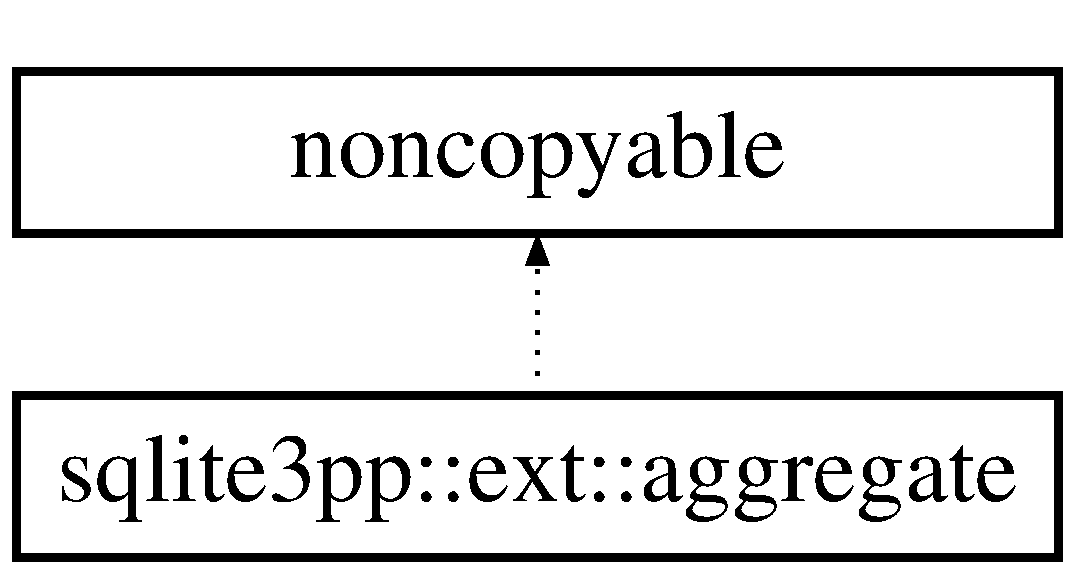
\includegraphics[height=2.000000cm]{classsqlite3pp_1_1ext_1_1aggregate}
\end{center}
\end{figure}
\subsection*{Public Types}
\begin{DoxyCompactItemize}
\item 
\hypertarget{classsqlite3pp_1_1ext_1_1aggregate_a42ce5bc3bb024595931764f2308f305e}{typedef boost\-::function$<$ void(\hyperlink{classsqlite3pp_1_1ext_1_1context}{context} \&)$>$ {\bfseries function\-\_\-handler}}\label{classsqlite3pp_1_1ext_1_1aggregate_a42ce5bc3bb024595931764f2308f305e}

\item 
\hypertarget{classsqlite3pp_1_1ext_1_1aggregate_a83211f4a5a9dfc213ff452245dde3d0d}{typedef boost\-::shared\-\_\-ptr\\*
$<$ boost\-::function\-\_\-base $>$ {\bfseries pfunction\-\_\-base}}\label{classsqlite3pp_1_1ext_1_1aggregate_a83211f4a5a9dfc213ff452245dde3d0d}

\end{DoxyCompactItemize}
\subsection*{Public Member Functions}
\begin{DoxyCompactItemize}
\item 
\hypertarget{classsqlite3pp_1_1ext_1_1aggregate_ad71d74c08c6d53328bab6bf1da0e625c}{{\bfseries aggregate} (\hyperlink{classsqlite3pp_1_1database}{database} \&db)}\label{classsqlite3pp_1_1ext_1_1aggregate_ad71d74c08c6d53328bab6bf1da0e625c}

\item 
\hypertarget{classsqlite3pp_1_1ext_1_1aggregate_a1274bb5675300d3f1d21155c6a259eea}{int {\bfseries create} (char const $\ast$name, function\-\_\-handler s, function\-\_\-handler f, int nargs=1)}\label{classsqlite3pp_1_1ext_1_1aggregate_a1274bb5675300d3f1d21155c6a259eea}

\item 
\hypertarget{classsqlite3pp_1_1ext_1_1aggregate_ab6b95557659b1cfeedf55a35558ef34c}{{\footnotesize template$<$class T $>$ }\\int {\bfseries create} (char const $\ast$name)}\label{classsqlite3pp_1_1ext_1_1aggregate_ab6b95557659b1cfeedf55a35558ef34c}

\item 
\hypertarget{classsqlite3pp_1_1ext_1_1aggregate_a2028d43621d1a5309a9218119f58ea09}{{\footnotesize template$<$class T , class P1 $>$ }\\int {\bfseries create} (char const $\ast$name)}\label{classsqlite3pp_1_1ext_1_1aggregate_a2028d43621d1a5309a9218119f58ea09}

\item 
\hypertarget{classsqlite3pp_1_1ext_1_1aggregate_a003fb5df884159eb6b39d6ae95212315}{{\footnotesize template$<$class T , class P1 , class P2 $>$ }\\int {\bfseries create} (char const $\ast$name)}\label{classsqlite3pp_1_1ext_1_1aggregate_a003fb5df884159eb6b39d6ae95212315}

\item 
\hypertarget{classsqlite3pp_1_1ext_1_1aggregate_af8160d679aa3aa7c78a1a4b15cb6832b}{{\footnotesize template$<$class T , class P1 , class P2 , class P3 $>$ }\\int {\bfseries create} (char const $\ast$name)}\label{classsqlite3pp_1_1ext_1_1aggregate_af8160d679aa3aa7c78a1a4b15cb6832b}

\item 
\hypertarget{classsqlite3pp_1_1ext_1_1aggregate_a70550b4815fd77a0d9a15f2738666376}{{\footnotesize template$<$class T , class P1 , class P2 , class P3 , class P4 $>$ }\\int {\bfseries create} (char const $\ast$name)}\label{classsqlite3pp_1_1ext_1_1aggregate_a70550b4815fd77a0d9a15f2738666376}

\item 
\hypertarget{classsqlite3pp_1_1ext_1_1aggregate_a02677f62769060c39b925f1997c2093d}{{\footnotesize template$<$class T , class P1 , class P2 , class P3 , class P4 , class P5 $>$ }\\int {\bfseries create} (char const $\ast$name)}\label{classsqlite3pp_1_1ext_1_1aggregate_a02677f62769060c39b925f1997c2093d}

\end{DoxyCompactItemize}


The documentation for this class was generated from the following files\-:\begin{DoxyCompactItemize}
\item 
sqlite3ppext.\-h\item 
sqlite3ppext.\-cpp\end{DoxyCompactItemize}

\hypertarget{classsqlite3pp_1_1command_1_1bindstream}{\section{sqlite3pp\-:\-:command\-:\-:bindstream Class Reference}
\label{classsqlite3pp_1_1command_1_1bindstream}\index{sqlite3pp\-::command\-::bindstream@{sqlite3pp\-::command\-::bindstream}}
}
\subsection*{Public Member Functions}
\begin{DoxyCompactItemize}
\item 
\hypertarget{classsqlite3pp_1_1command_1_1bindstream_ad57cb71ac6884312b455557633a25854}{{\bfseries bindstream} (\hyperlink{classsqlite3pp_1_1command}{command} \&cmd, int idx)}\label{classsqlite3pp_1_1command_1_1bindstream_ad57cb71ac6884312b455557633a25854}

\item 
\hypertarget{classsqlite3pp_1_1command_1_1bindstream_abaaf836396249baededca17a894e20ae}{{\footnotesize template$<$class T $>$ }\\\hyperlink{classsqlite3pp_1_1command_1_1bindstream}{bindstream} \& {\bfseries operator$<$$<$} (T value)}\label{classsqlite3pp_1_1command_1_1bindstream_abaaf836396249baededca17a894e20ae}

\end{DoxyCompactItemize}


The documentation for this class was generated from the following files\-:\begin{DoxyCompactItemize}
\item 
sqlite3pp.\-h\item 
sqlite3pp.\-cpp\end{DoxyCompactItemize}

\hypertarget{classsqlite3pp_1_1command}{\section{sqlite3pp\-:\-:command Class Reference}
\label{classsqlite3pp_1_1command}\index{sqlite3pp\-::command@{sqlite3pp\-::command}}
}
Inheritance diagram for sqlite3pp\-:\-:command\-:\begin{figure}[H]
\begin{center}
\leavevmode
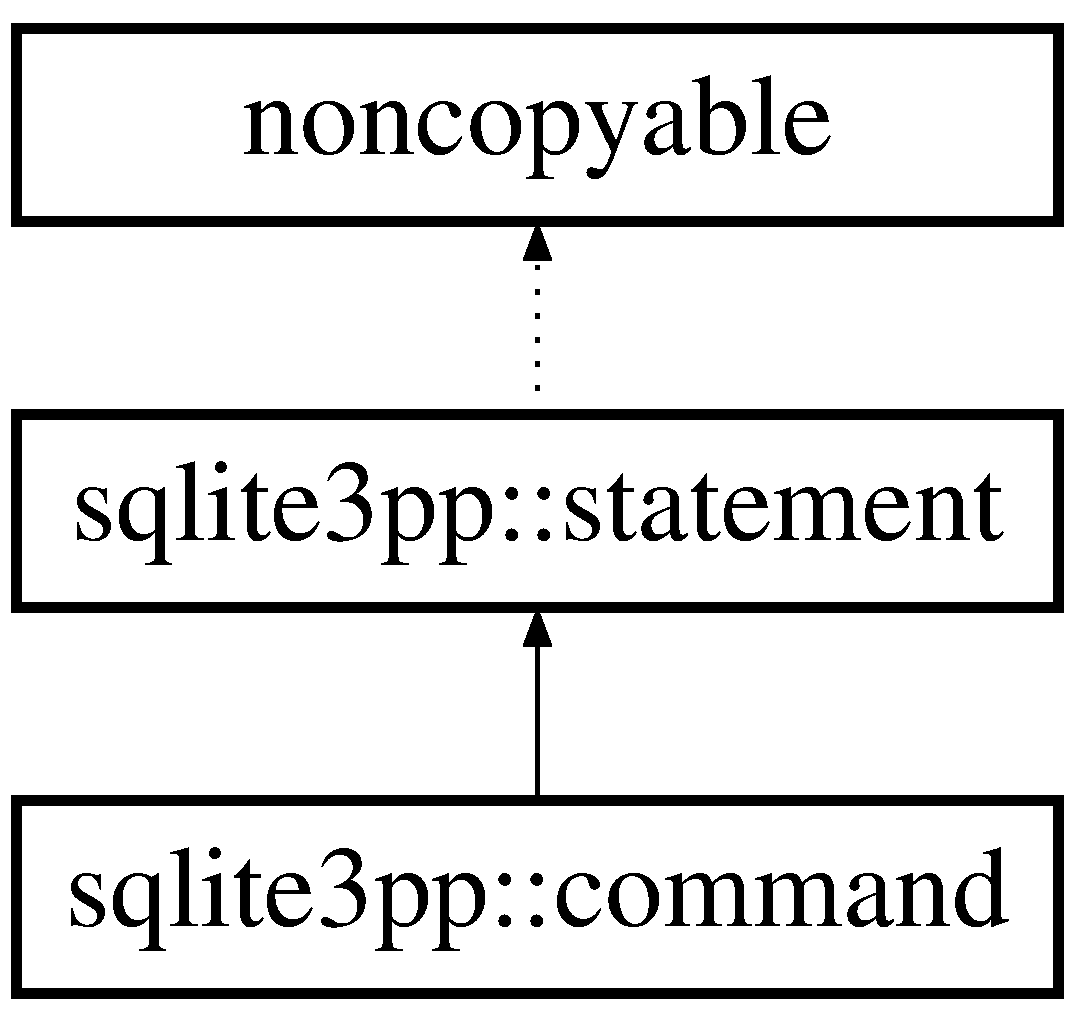
\includegraphics[height=3.000000cm]{classsqlite3pp_1_1command}
\end{center}
\end{figure}
\subsection*{Classes}
\begin{DoxyCompactItemize}
\item 
class \hyperlink{classsqlite3pp_1_1command_1_1bindstream}{bindstream}
\end{DoxyCompactItemize}
\subsection*{Public Member Functions}
\begin{DoxyCompactItemize}
\item 
\hypertarget{classsqlite3pp_1_1command_a25816f7a1f3825982fddbcbb5bb086f0}{{\bfseries command} (\hyperlink{classsqlite3pp_1_1database}{database} \&db, char const $\ast$stmt=0)}\label{classsqlite3pp_1_1command_a25816f7a1f3825982fddbcbb5bb086f0}

\item 
\hypertarget{classsqlite3pp_1_1command_aa2754e08a750704e08d8fe1cc0edaba8}{\hyperlink{classsqlite3pp_1_1command_1_1bindstream}{bindstream} {\bfseries binder} (int idx=1)}\label{classsqlite3pp_1_1command_aa2754e08a750704e08d8fe1cc0edaba8}

\item 
\hypertarget{classsqlite3pp_1_1command_adcc7aae09d6c10448cb7436621fd3417}{int {\bfseries execute} ()}\label{classsqlite3pp_1_1command_adcc7aae09d6c10448cb7436621fd3417}

\item 
\hypertarget{classsqlite3pp_1_1command_a8ea7613b0b8023124f3a85c0553042e0}{int {\bfseries execute\-\_\-all} ()}\label{classsqlite3pp_1_1command_a8ea7613b0b8023124f3a85c0553042e0}

\end{DoxyCompactItemize}
\subsection*{Additional Inherited Members}


The documentation for this class was generated from the following files\-:\begin{DoxyCompactItemize}
\item 
sqlite3pp.\-h\item 
sqlite3pp.\-cpp\end{DoxyCompactItemize}

\hypertarget{classsqlite3pp_1_1ext_1_1context}{\section{sqlite3pp\-:\-:ext\-:\-:context Class Reference}
\label{classsqlite3pp_1_1ext_1_1context}\index{sqlite3pp\-::ext\-::context@{sqlite3pp\-::ext\-::context}}
}
Inheritance diagram for sqlite3pp\-:\-:ext\-:\-:context\-:\begin{figure}[H]
\begin{center}
\leavevmode
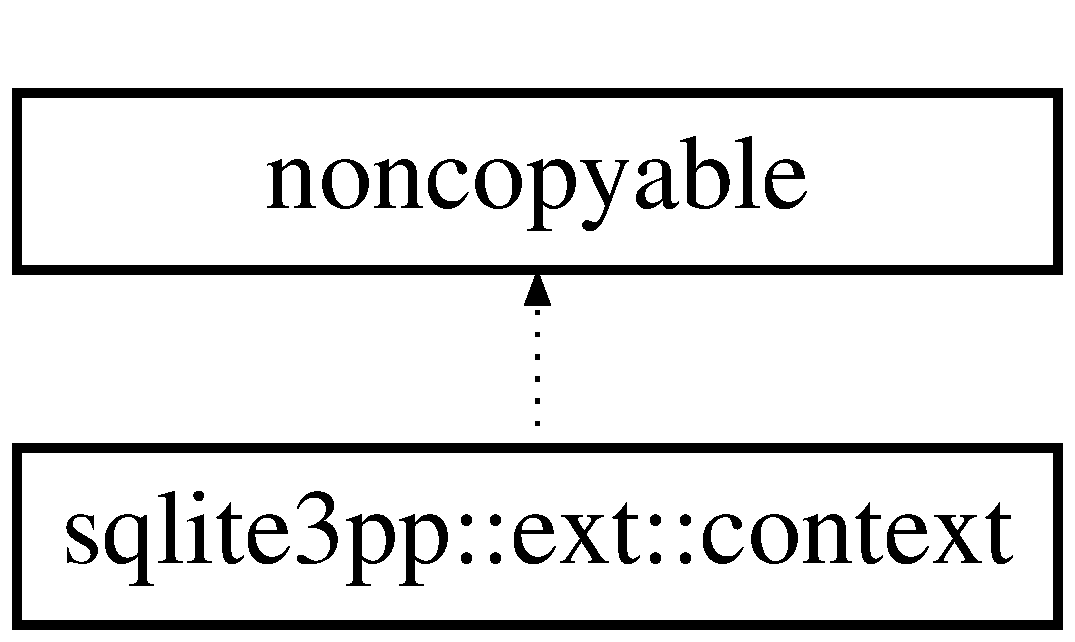
\includegraphics[height=2.000000cm]{classsqlite3pp_1_1ext_1_1context}
\end{center}
\end{figure}
\subsection*{Public Member Functions}
\begin{DoxyCompactItemize}
\item 
\hypertarget{classsqlite3pp_1_1ext_1_1context_a77154187b26ae1e8d7ba201473ff69e9}{{\bfseries context} (sqlite3\-\_\-context $\ast$ctx, int nargs=0, sqlite3\-\_\-value $\ast$$\ast$values=0)}\label{classsqlite3pp_1_1ext_1_1context_a77154187b26ae1e8d7ba201473ff69e9}

\item 
\hypertarget{classsqlite3pp_1_1ext_1_1context_a26bec66b424da39bcb56fbef411eece0}{int {\bfseries args\-\_\-count} () const }\label{classsqlite3pp_1_1ext_1_1context_a26bec66b424da39bcb56fbef411eece0}

\item 
\hypertarget{classsqlite3pp_1_1ext_1_1context_a56b57178738812292492c085eeb762b1}{int {\bfseries args\-\_\-bytes} (int idx) const }\label{classsqlite3pp_1_1ext_1_1context_a56b57178738812292492c085eeb762b1}

\item 
\hypertarget{classsqlite3pp_1_1ext_1_1context_a5f8efbc64463809b39cf300c101937a5}{int {\bfseries args\-\_\-type} (int idx) const }\label{classsqlite3pp_1_1ext_1_1context_a5f8efbc64463809b39cf300c101937a5}

\item 
\hypertarget{classsqlite3pp_1_1ext_1_1context_a7dee5517eabd76630ce46dbc6ee053bb}{{\footnotesize template$<$class T $>$ }\\T {\bfseries get} (int idx) const }\label{classsqlite3pp_1_1ext_1_1context_a7dee5517eabd76630ce46dbc6ee053bb}

\item 
\hypertarget{classsqlite3pp_1_1ext_1_1context_addc69b54f36d40cb302671b7bd8a64dc}{void {\bfseries result} (int value)}\label{classsqlite3pp_1_1ext_1_1context_addc69b54f36d40cb302671b7bd8a64dc}

\item 
\hypertarget{classsqlite3pp_1_1ext_1_1context_a70250ebb8256611efe70e1f0bf4b7364}{void {\bfseries result} (double value)}\label{classsqlite3pp_1_1ext_1_1context_a70250ebb8256611efe70e1f0bf4b7364}

\item 
\hypertarget{classsqlite3pp_1_1ext_1_1context_a75250069330291844e64b422711bbd37}{void {\bfseries result} (long long int value)}\label{classsqlite3pp_1_1ext_1_1context_a75250069330291844e64b422711bbd37}

\item 
\hypertarget{classsqlite3pp_1_1ext_1_1context_a068c74a26a53283916919a67139a60e0}{void {\bfseries result} (std\-::string const \&value)}\label{classsqlite3pp_1_1ext_1_1context_a068c74a26a53283916919a67139a60e0}

\item 
\hypertarget{classsqlite3pp_1_1ext_1_1context_a051c2ca3865cca1a584fdd0f805245b5}{void {\bfseries result} (char const $\ast$value, bool fstatic=true)}\label{classsqlite3pp_1_1ext_1_1context_a051c2ca3865cca1a584fdd0f805245b5}

\item 
\hypertarget{classsqlite3pp_1_1ext_1_1context_a10845cffae213febaeaadab7f53442a0}{void {\bfseries result} (void const $\ast$value, int n, bool fstatic=true)}\label{classsqlite3pp_1_1ext_1_1context_a10845cffae213febaeaadab7f53442a0}

\item 
\hypertarget{classsqlite3pp_1_1ext_1_1context_aa72765ff4f1f6618379ff8a27f532e57}{void {\bfseries result} ()}\label{classsqlite3pp_1_1ext_1_1context_aa72765ff4f1f6618379ff8a27f532e57}

\item 
\hypertarget{classsqlite3pp_1_1ext_1_1context_a7a4b071b8b70c962b35336d7ed554d7c}{void {\bfseries result} (\hyperlink{classsqlite3pp_1_1null__type}{null\-\_\-type})}\label{classsqlite3pp_1_1ext_1_1context_a7a4b071b8b70c962b35336d7ed554d7c}

\item 
\hypertarget{classsqlite3pp_1_1ext_1_1context_a7da6fea6eaa62c9f3723fdcee1d7ce5d}{void {\bfseries result\-\_\-copy} (int idx)}\label{classsqlite3pp_1_1ext_1_1context_a7da6fea6eaa62c9f3723fdcee1d7ce5d}

\item 
\hypertarget{classsqlite3pp_1_1ext_1_1context_aff50f7fc48fd1988ca3b3550072eb10a}{void {\bfseries result\-\_\-error} (char const $\ast$msg)}\label{classsqlite3pp_1_1ext_1_1context_aff50f7fc48fd1988ca3b3550072eb10a}

\item 
\hypertarget{classsqlite3pp_1_1ext_1_1context_a6c858075387a36360564f8f763ab2045}{void $\ast$ {\bfseries aggregate\-\_\-data} (int size)}\label{classsqlite3pp_1_1ext_1_1context_a6c858075387a36360564f8f763ab2045}

\item 
\hypertarget{classsqlite3pp_1_1ext_1_1context_a7b90abdc58b9cc33062d1882e41c4dc0}{int {\bfseries aggregate\-\_\-count} ()}\label{classsqlite3pp_1_1ext_1_1context_a7b90abdc58b9cc33062d1882e41c4dc0}

\end{DoxyCompactItemize}


The documentation for this class was generated from the following files\-:\begin{DoxyCompactItemize}
\item 
sqlite3ppext.\-h\item 
sqlite3ppext.\-cpp\end{DoxyCompactItemize}

\hypertarget{classsqlite3pp_1_1database}{\section{sqlite3pp\-:\-:database Class Reference}
\label{classsqlite3pp_1_1database}\index{sqlite3pp\-::database@{sqlite3pp\-::database}}
}
Inheritance diagram for sqlite3pp\-:\-:database\-:\begin{figure}[H]
\begin{center}
\leavevmode
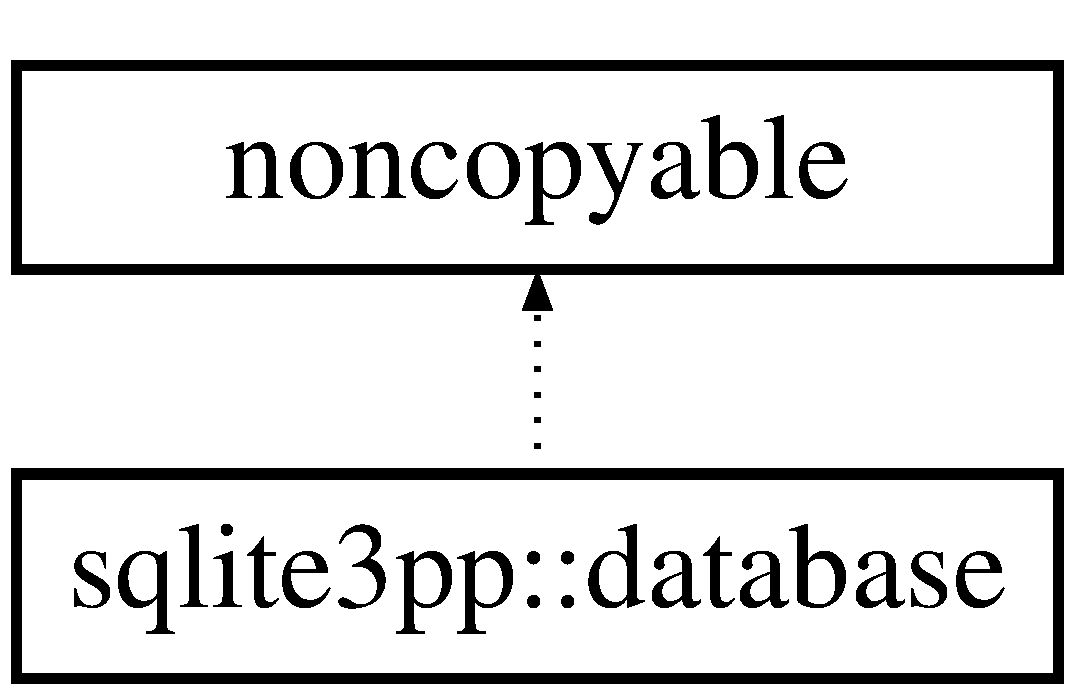
\includegraphics[height=2.000000cm]{classsqlite3pp_1_1database}
\end{center}
\end{figure}
\subsection*{Public Types}
\begin{DoxyCompactItemize}
\item 
\hypertarget{classsqlite3pp_1_1database_a00e316167d2a96f2458372e12e7dc9ac}{typedef boost\-::function$<$ int(int)$>$ {\bfseries busy\-\_\-handler}}\label{classsqlite3pp_1_1database_a00e316167d2a96f2458372e12e7dc9ac}

\item 
\hypertarget{classsqlite3pp_1_1database_ab813e24d10edc9c24102b3f2459be6a2}{typedef boost\-::function$<$ int()$>$ {\bfseries commit\-\_\-handler}}\label{classsqlite3pp_1_1database_ab813e24d10edc9c24102b3f2459be6a2}

\item 
\hypertarget{classsqlite3pp_1_1database_a307b494852597cbe1baaef1197c1ecb4}{typedef boost\-::function$<$ void()$>$ {\bfseries rollback\-\_\-handler}}\label{classsqlite3pp_1_1database_a307b494852597cbe1baaef1197c1ecb4}

\item 
\hypertarget{classsqlite3pp_1_1database_a86dc0ab97b10669c75e7b35480e8666a}{typedef boost\-::function$<$ void(int, \\*
char const $\ast$, char const \\*
$\ast$, long long int)$>$ {\bfseries update\-\_\-handler}}\label{classsqlite3pp_1_1database_a86dc0ab97b10669c75e7b35480e8666a}

\item 
\hypertarget{classsqlite3pp_1_1database_a29502faa9cba0fd03cf08d8815fc714e}{typedef boost\-::function$<$ int(int, \\*
char const $\ast$, char const \\*
$\ast$, char const $\ast$, char const $\ast$)$>$ {\bfseries authorize\-\_\-handler}}\label{classsqlite3pp_1_1database_a29502faa9cba0fd03cf08d8815fc714e}

\end{DoxyCompactItemize}
\subsection*{Public Member Functions}
\begin{DoxyCompactItemize}
\item 
\hypertarget{classsqlite3pp_1_1database_ad82d2544bdc21484b1ad5ba1744224ee}{{\bfseries database} (char const $\ast$dbname=0)}\label{classsqlite3pp_1_1database_ad82d2544bdc21484b1ad5ba1744224ee}

\item 
\hypertarget{classsqlite3pp_1_1database_a84b8252faa02ddd1f49b41b065ae8bcb}{int {\bfseries connect} (char const $\ast$dbname)}\label{classsqlite3pp_1_1database_a84b8252faa02ddd1f49b41b065ae8bcb}

\item 
\hypertarget{classsqlite3pp_1_1database_ac52e19d2ca06314cb027dccbf78f2f70}{int {\bfseries connect\-\_\-v2} (char const $\ast$dbname, int flags, char const $\ast$vfs=0)}\label{classsqlite3pp_1_1database_ac52e19d2ca06314cb027dccbf78f2f70}

\item 
\hypertarget{classsqlite3pp_1_1database_a51227d51ba00357d093588ce7a9387c8}{int {\bfseries disconnect} ()}\label{classsqlite3pp_1_1database_a51227d51ba00357d093588ce7a9387c8}

\item 
\hypertarget{classsqlite3pp_1_1database_a1997005540b310306af57ce11da52964}{int {\bfseries attach} (char const $\ast$dbname, char const $\ast$name)}\label{classsqlite3pp_1_1database_a1997005540b310306af57ce11da52964}

\item 
\hypertarget{classsqlite3pp_1_1database_a54c017665849c1441595a9a3eb337011}{int {\bfseries detach} (char const $\ast$name)}\label{classsqlite3pp_1_1database_a54c017665849c1441595a9a3eb337011}

\item 
\hypertarget{classsqlite3pp_1_1database_af27c4fa34418d2af3735d195baa5b281}{long long int {\bfseries last\-\_\-insert\-\_\-rowid} () const }\label{classsqlite3pp_1_1database_af27c4fa34418d2af3735d195baa5b281}

\item 
\hypertarget{classsqlite3pp_1_1database_a8ba2facb29ad175924269b78a2970e6d}{int {\bfseries error\-\_\-code} () const }\label{classsqlite3pp_1_1database_a8ba2facb29ad175924269b78a2970e6d}

\item 
\hypertarget{classsqlite3pp_1_1database_a5b77f2e8faa87bd6512f1da3b1149b6a}{char const $\ast$ {\bfseries error\-\_\-msg} () const }\label{classsqlite3pp_1_1database_a5b77f2e8faa87bd6512f1da3b1149b6a}

\item 
\hypertarget{classsqlite3pp_1_1database_aef941b972df875ba2a5062d324c72a7a}{int {\bfseries execute} (char const $\ast$sql)}\label{classsqlite3pp_1_1database_aef941b972df875ba2a5062d324c72a7a}

\item 
\hypertarget{classsqlite3pp_1_1database_a19fbbc61f8fd5b398f904d343c1c27a9}{int {\bfseries executef} (char const $\ast$sql,...)}\label{classsqlite3pp_1_1database_a19fbbc61f8fd5b398f904d343c1c27a9}

\item 
\hypertarget{classsqlite3pp_1_1database_aeace5855fa4540a6716321c2af0499bd}{int {\bfseries set\-\_\-busy\-\_\-timeout} (int ms)}\label{classsqlite3pp_1_1database_aeace5855fa4540a6716321c2af0499bd}

\item 
\hypertarget{classsqlite3pp_1_1database_adf5482aa554f0e4612d3ba83cbde6d7c}{void {\bfseries set\-\_\-busy\-\_\-handler} (busy\-\_\-handler h)}\label{classsqlite3pp_1_1database_adf5482aa554f0e4612d3ba83cbde6d7c}

\item 
\hypertarget{classsqlite3pp_1_1database_aec8828634ab248e318d9605cbafaac2a}{void {\bfseries set\-\_\-commit\-\_\-handler} (commit\-\_\-handler h)}\label{classsqlite3pp_1_1database_aec8828634ab248e318d9605cbafaac2a}

\item 
\hypertarget{classsqlite3pp_1_1database_a02558b73420568fa8f0199da031b13e6}{void {\bfseries set\-\_\-rollback\-\_\-handler} (rollback\-\_\-handler h)}\label{classsqlite3pp_1_1database_a02558b73420568fa8f0199da031b13e6}

\item 
\hypertarget{classsqlite3pp_1_1database_aa0ce424227761d27a4633375f8e309f4}{void {\bfseries set\-\_\-update\-\_\-handler} (update\-\_\-handler h)}\label{classsqlite3pp_1_1database_aa0ce424227761d27a4633375f8e309f4}

\item 
\hypertarget{classsqlite3pp_1_1database_ab5b1c02d58c555c5889d29c3ae8535b4}{void {\bfseries set\-\_\-authorize\-\_\-handler} (authorize\-\_\-handler h)}\label{classsqlite3pp_1_1database_ab5b1c02d58c555c5889d29c3ae8535b4}

\end{DoxyCompactItemize}
\subsection*{Friends}
\begin{DoxyCompactItemize}
\item 
\hypertarget{classsqlite3pp_1_1database_a4682195a7dfc5da7346d8cfadcf0eb20}{class {\bfseries statement}}\label{classsqlite3pp_1_1database_a4682195a7dfc5da7346d8cfadcf0eb20}

\item 
\hypertarget{classsqlite3pp_1_1database_a76d8b698f6b190905b6c9f75fc581f93}{class {\bfseries database\-\_\-error}}\label{classsqlite3pp_1_1database_a76d8b698f6b190905b6c9f75fc581f93}

\item 
\hypertarget{classsqlite3pp_1_1database_a0af2b37d4b82567629796c72049d6e6e}{class {\bfseries ext\-::function}}\label{classsqlite3pp_1_1database_a0af2b37d4b82567629796c72049d6e6e}

\item 
\hypertarget{classsqlite3pp_1_1database_a3daeb4aba0850368a48e8024f05d4863}{class {\bfseries ext\-::aggregate}}\label{classsqlite3pp_1_1database_a3daeb4aba0850368a48e8024f05d4863}

\end{DoxyCompactItemize}


The documentation for this class was generated from the following files\-:\begin{DoxyCompactItemize}
\item 
sqlite3pp.\-h\item 
sqlite3pp.\-cpp\end{DoxyCompactItemize}

\hypertarget{classsqlite3pp_1_1database__error}{\section{sqlite3pp\-:\-:database\-\_\-error Class Reference}
\label{classsqlite3pp_1_1database__error}\index{sqlite3pp\-::database\-\_\-error@{sqlite3pp\-::database\-\_\-error}}
}
Inheritance diagram for sqlite3pp\-:\-:database\-\_\-error\-:\begin{figure}[H]
\begin{center}
\leavevmode
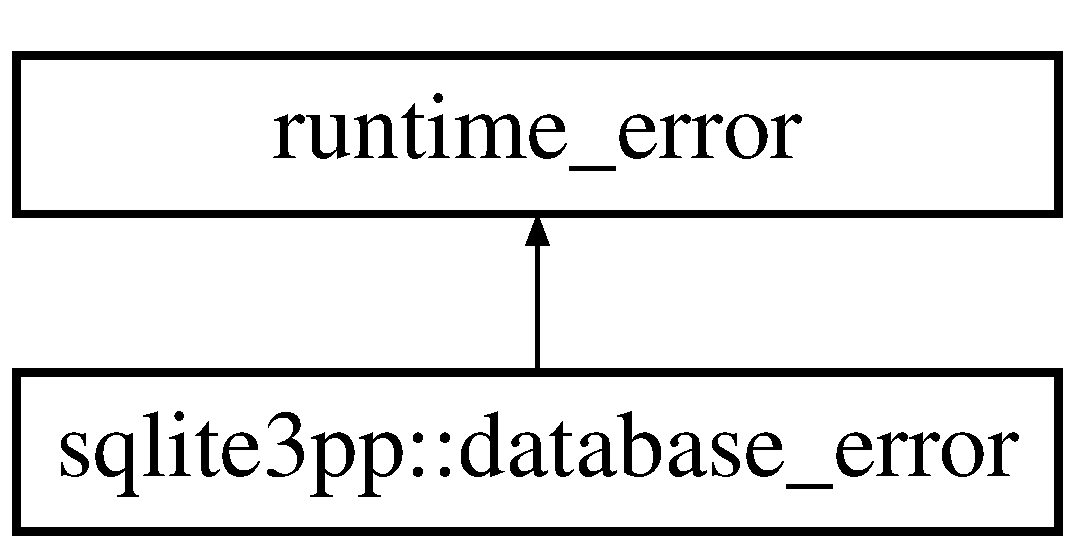
\includegraphics[height=2.000000cm]{classsqlite3pp_1_1database__error}
\end{center}
\end{figure}
\subsection*{Public Member Functions}
\begin{DoxyCompactItemize}
\item 
\hypertarget{classsqlite3pp_1_1database__error_a38aeb58dbf02b6f668c6df08a1932b1a}{{\bfseries database\-\_\-error} (char const $\ast$msg)}\label{classsqlite3pp_1_1database__error_a38aeb58dbf02b6f668c6df08a1932b1a}

\item 
\hypertarget{classsqlite3pp_1_1database__error_a03789ebe1ee0fdecb8e50ba728b650e8}{{\bfseries database\-\_\-error} (\hyperlink{classsqlite3pp_1_1database}{database} \&db)}\label{classsqlite3pp_1_1database__error_a03789ebe1ee0fdecb8e50ba728b650e8}

\end{DoxyCompactItemize}


The documentation for this class was generated from the following files\-:\begin{DoxyCompactItemize}
\item 
sqlite3pp.\-h\item 
sqlite3pp.\-cpp\end{DoxyCompactItemize}

\hypertarget{class_database_manager}{\section{Database\-Manager Class Reference}
\label{class_database_manager}\index{Database\-Manager@{Database\-Manager}}
}


Database Manager class.  




{\ttfamily \#include $<$Database\-Manager.\-h$>$}

\subsection*{Public Member Functions}
\begin{DoxyCompactItemize}
\item 
\hyperlink{class_database_manager_a24e3c3701ce01fdac96cc170b334aeba}{Database\-Manager} (std\-::string filepath)
\begin{DoxyCompactList}\small\item\em Class Constructor. \end{DoxyCompactList}\item 
\hyperlink{class_database_manager_ae9b3a5da1e04fbb00faf8a034da1d063}{$\sim$\-Database\-Manager} ()
\begin{DoxyCompactList}\small\item\em Class Destructor. \end{DoxyCompactList}\item 
std\-::vector$<$ \hyperlink{class_texto}{Texto} $\ast$ $>$ \hyperlink{class_database_manager_a362dc9fb3beb6cd0ca9cb1d42703ec03}{get\-\_\-textos} ()
\begin{DoxyCompactList}\small\item\em The getter for the texts. \end{DoxyCompactList}\item 
void \hyperlink{class_database_manager_a3ea3390feb2069715c7af51ebb41a26c}{get\-\_\-textos\-\_\-by\-\_\-type} (std\-::vector$<$ \hyperlink{class_texto_tecnico}{Texto\-Tecnico} $\ast$ $>$ \&textos\-\_\-tecnicos, std\-::vector$<$ \hyperlink{class_texto_literario}{Texto\-Literario} $\ast$ $>$ \&textos\-\_\-literarios, std\-::vector$<$ \hyperlink{class_texto_noticioso}{Texto\-Noticioso} $\ast$ $>$ \&textos\-\_\-noticiosos)
\begin{DoxyCompactList}\small\item\em A getter for the texts, separated by type vectors. \end{DoxyCompactList}\item 
std\-::vector$<$ \hyperlink{class_tradutor}{Tradutor} $\ast$ $>$ \hyperlink{class_database_manager_ad0f509067821ad15a9b25d86d2b515a4}{get\-\_\-tradutores} ()
\begin{DoxyCompactList}\small\item\em The getter for the translators. \end{DoxyCompactList}\item 
std\-::vector$<$ \hyperlink{class_encomenda}{Encomenda} $\ast$ $>$ \hyperlink{class_database_manager_a5c2b2ad77ee83de5b1fb2f07cdfc6736}{get\-\_\-encomendas} ()
\begin{DoxyCompactList}\small\item\em The getter for the orders. \end{DoxyCompactList}\item 
bool \hyperlink{class_database_manager_a10e0b6e056bcc0b669e272b839ae92fe}{create\-\_\-update\-\_\-record} (\hyperlink{class_texto}{Texto} $\ast$texto)
\begin{DoxyCompactList}\small\item\em Creates a new record or updates an existing one. \end{DoxyCompactList}\item 
bool \hyperlink{class_database_manager_aedc255310da21463f3297f3333898605}{delete\-\_\-record} (\hyperlink{class_texto}{Texto} $\ast$texto)
\begin{DoxyCompactList}\small\item\em Deletes an existing record. \end{DoxyCompactList}\item 
bool \hyperlink{class_database_manager_a587389f45912fee630df72658a4d09b0}{create\-\_\-update\-\_\-record} (\hyperlink{class_tradutor}{Tradutor} $\ast$tradutor)
\begin{DoxyCompactList}\small\item\em Creates a new record or updates an existing one. \end{DoxyCompactList}\item 
bool \hyperlink{class_database_manager_a861c8ab275b7d9e100ebb71889578c40}{delete\-\_\-record} (\hyperlink{class_tradutor}{Tradutor} $\ast$tradutor)
\begin{DoxyCompactList}\small\item\em Deletes an existing record. \end{DoxyCompactList}\item 
bool \hyperlink{class_database_manager_a10fd54af873e6902a3a6ee45f71eb42c}{create\-\_\-update\-\_\-record} (\hyperlink{class_encomenda}{Encomenda} $\ast$encomenda)
\begin{DoxyCompactList}\small\item\em Creates a new record or updates an existing one. \end{DoxyCompactList}\item 
bool \hyperlink{class_database_manager_aa78e5396d0be88098a97703f31fb72ec}{delete\-\_\-record} (\hyperlink{class_encomenda}{Encomenda} $\ast$encomenda)
\begin{DoxyCompactList}\small\item\em Deletes an existing record. \end{DoxyCompactList}\item 
unsigned int \hyperlink{class_database_manager_a5af3db3952fc2af64a43fd0403138c04}{get\-\_\-maior\-\_\-id} (\hyperlink{_database_manager_8h_ad36b2b2507c9846942e0b412d07e5438}{k\-Class} asker)
\begin{DoxyCompactList}\small\item\em Returns the biggest I\-D record for a class type. \end{DoxyCompactList}\end{DoxyCompactItemize}


\subsection{Detailed Description}
Database Manager class. 

This class handles all the I\-O to the database (with some helper functions). 

\subsection{Constructor \& Destructor Documentation}
\hypertarget{class_database_manager_a24e3c3701ce01fdac96cc170b334aeba}{\index{Database\-Manager@{Database\-Manager}!Database\-Manager@{Database\-Manager}}
\index{Database\-Manager@{Database\-Manager}!DatabaseManager@{Database\-Manager}}
\subsubsection[{Database\-Manager}]{\setlength{\rightskip}{0pt plus 5cm}Database\-Manager\-::\-Database\-Manager (
\begin{DoxyParamCaption}
\item[{std\-::string}]{filepath}
\end{DoxyParamCaption}
)}}\label{class_database_manager_a24e3c3701ce01fdac96cc170b334aeba}


Class Constructor. 


\begin{DoxyParams}{Parameters}
{\em filepath} & The path for the sqlite3 database file. If a file doesn't exist at target, a new one will be created and initialized. \\
\hline
\end{DoxyParams}
\hypertarget{class_database_manager_ae9b3a5da1e04fbb00faf8a034da1d063}{\index{Database\-Manager@{Database\-Manager}!$\sim$\-Database\-Manager@{$\sim$\-Database\-Manager}}
\index{$\sim$\-Database\-Manager@{$\sim$\-Database\-Manager}!DatabaseManager@{Database\-Manager}}
\subsubsection[{$\sim$\-Database\-Manager}]{\setlength{\rightskip}{0pt plus 5cm}Database\-Manager\-::$\sim$\-Database\-Manager (
\begin{DoxyParamCaption}
{}
\end{DoxyParamCaption}
)}}\label{class_database_manager_ae9b3a5da1e04fbb00faf8a034da1d063}


Class Destructor. 



\subsection{Member Function Documentation}
\hypertarget{class_database_manager_a10e0b6e056bcc0b669e272b839ae92fe}{\index{Database\-Manager@{Database\-Manager}!create\-\_\-update\-\_\-record@{create\-\_\-update\-\_\-record}}
\index{create\-\_\-update\-\_\-record@{create\-\_\-update\-\_\-record}!DatabaseManager@{Database\-Manager}}
\subsubsection[{create\-\_\-update\-\_\-record}]{\setlength{\rightskip}{0pt plus 5cm}bool Database\-Manager\-::create\-\_\-update\-\_\-record (
\begin{DoxyParamCaption}
\item[{{\bf Texto} $\ast$}]{texto}
\end{DoxyParamCaption}
)}}\label{class_database_manager_a10e0b6e056bcc0b669e272b839ae92fe}


Creates a new record or updates an existing one. 


\begin{DoxyParams}{Parameters}
{\em texto} & The text to be saved. \\
\hline
\end{DoxyParams}
\begin{DoxyReturn}{Returns}
true on success, false on error. 
\end{DoxyReturn}
\hypertarget{class_database_manager_a587389f45912fee630df72658a4d09b0}{\index{Database\-Manager@{Database\-Manager}!create\-\_\-update\-\_\-record@{create\-\_\-update\-\_\-record}}
\index{create\-\_\-update\-\_\-record@{create\-\_\-update\-\_\-record}!DatabaseManager@{Database\-Manager}}
\subsubsection[{create\-\_\-update\-\_\-record}]{\setlength{\rightskip}{0pt plus 5cm}bool Database\-Manager\-::create\-\_\-update\-\_\-record (
\begin{DoxyParamCaption}
\item[{{\bf Tradutor} $\ast$}]{tradutor}
\end{DoxyParamCaption}
)}}\label{class_database_manager_a587389f45912fee630df72658a4d09b0}


Creates a new record or updates an existing one. 


\begin{DoxyParams}{Parameters}
{\em tradutor} & The translator to be saved. \\
\hline
\end{DoxyParams}
\begin{DoxyReturn}{Returns}
true on success, false on error. 
\end{DoxyReturn}
\hypertarget{class_database_manager_a10fd54af873e6902a3a6ee45f71eb42c}{\index{Database\-Manager@{Database\-Manager}!create\-\_\-update\-\_\-record@{create\-\_\-update\-\_\-record}}
\index{create\-\_\-update\-\_\-record@{create\-\_\-update\-\_\-record}!DatabaseManager@{Database\-Manager}}
\subsubsection[{create\-\_\-update\-\_\-record}]{\setlength{\rightskip}{0pt plus 5cm}bool Database\-Manager\-::create\-\_\-update\-\_\-record (
\begin{DoxyParamCaption}
\item[{{\bf Encomenda} $\ast$}]{encomenda}
\end{DoxyParamCaption}
)}}\label{class_database_manager_a10fd54af873e6902a3a6ee45f71eb42c}


Creates a new record or updates an existing one. 


\begin{DoxyParams}{Parameters}
{\em encomenda} & The order to be saved. \\
\hline
\end{DoxyParams}
\begin{DoxyReturn}{Returns}
true on success, false on error. 
\end{DoxyReturn}
\hypertarget{class_database_manager_aedc255310da21463f3297f3333898605}{\index{Database\-Manager@{Database\-Manager}!delete\-\_\-record@{delete\-\_\-record}}
\index{delete\-\_\-record@{delete\-\_\-record}!DatabaseManager@{Database\-Manager}}
\subsubsection[{delete\-\_\-record}]{\setlength{\rightskip}{0pt plus 5cm}bool Database\-Manager\-::delete\-\_\-record (
\begin{DoxyParamCaption}
\item[{{\bf Texto} $\ast$}]{texto}
\end{DoxyParamCaption}
)}}\label{class_database_manager_aedc255310da21463f3297f3333898605}


Deletes an existing record. 


\begin{DoxyParams}{Parameters}
{\em texto} & The text to be deleted. \\
\hline
\end{DoxyParams}
\begin{DoxyReturn}{Returns}
true on success, false on error. 
\end{DoxyReturn}
\hypertarget{class_database_manager_a861c8ab275b7d9e100ebb71889578c40}{\index{Database\-Manager@{Database\-Manager}!delete\-\_\-record@{delete\-\_\-record}}
\index{delete\-\_\-record@{delete\-\_\-record}!DatabaseManager@{Database\-Manager}}
\subsubsection[{delete\-\_\-record}]{\setlength{\rightskip}{0pt plus 5cm}bool Database\-Manager\-::delete\-\_\-record (
\begin{DoxyParamCaption}
\item[{{\bf Tradutor} $\ast$}]{tradutor}
\end{DoxyParamCaption}
)}}\label{class_database_manager_a861c8ab275b7d9e100ebb71889578c40}


Deletes an existing record. 


\begin{DoxyParams}{Parameters}
{\em tradutor} & The translator to be deleted. \\
\hline
\end{DoxyParams}
\begin{DoxyReturn}{Returns}
true on success, false on error. 
\end{DoxyReturn}
\hypertarget{class_database_manager_aa78e5396d0be88098a97703f31fb72ec}{\index{Database\-Manager@{Database\-Manager}!delete\-\_\-record@{delete\-\_\-record}}
\index{delete\-\_\-record@{delete\-\_\-record}!DatabaseManager@{Database\-Manager}}
\subsubsection[{delete\-\_\-record}]{\setlength{\rightskip}{0pt plus 5cm}bool Database\-Manager\-::delete\-\_\-record (
\begin{DoxyParamCaption}
\item[{{\bf Encomenda} $\ast$}]{encomenda}
\end{DoxyParamCaption}
)}}\label{class_database_manager_aa78e5396d0be88098a97703f31fb72ec}


Deletes an existing record. 


\begin{DoxyParams}{Parameters}
{\em encomenda} & The order to be deleted. \\
\hline
\end{DoxyParams}
\begin{DoxyReturn}{Returns}
true on success, false on error. 
\end{DoxyReturn}
\hypertarget{class_database_manager_a5c2b2ad77ee83de5b1fb2f07cdfc6736}{\index{Database\-Manager@{Database\-Manager}!get\-\_\-encomendas@{get\-\_\-encomendas}}
\index{get\-\_\-encomendas@{get\-\_\-encomendas}!DatabaseManager@{Database\-Manager}}
\subsubsection[{get\-\_\-encomendas}]{\setlength{\rightskip}{0pt plus 5cm}std\-::vector$<$ {\bf Encomenda} $\ast$ $>$ Database\-Manager\-::get\-\_\-encomendas (
\begin{DoxyParamCaption}
{}
\end{DoxyParamCaption}
)}}\label{class_database_manager_a5c2b2ad77ee83de5b1fb2f07cdfc6736}


The getter for the orders. 

\begin{DoxyReturn}{Returns}
A vector with all the orders (as \hyperlink{class_encomenda}{Encomenda} object pointers). 
\end{DoxyReturn}
\hypertarget{class_database_manager_a5af3db3952fc2af64a43fd0403138c04}{\index{Database\-Manager@{Database\-Manager}!get\-\_\-maior\-\_\-id@{get\-\_\-maior\-\_\-id}}
\index{get\-\_\-maior\-\_\-id@{get\-\_\-maior\-\_\-id}!DatabaseManager@{Database\-Manager}}
\subsubsection[{get\-\_\-maior\-\_\-id}]{\setlength{\rightskip}{0pt plus 5cm}unsigned int Database\-Manager\-::get\-\_\-maior\-\_\-id (
\begin{DoxyParamCaption}
\item[{{\bf k\-Class}}]{asker}
\end{DoxyParamCaption}
)}}\label{class_database_manager_a5af3db3952fc2af64a43fd0403138c04}


Returns the biggest I\-D record for a class type. 


\begin{DoxyParams}{Parameters}
{\em k\-Class} & The class as defined on the Class enum. \\
\hline
\end{DoxyParams}
\begin{DoxySeeAlso}{See Also}
Class enum 
\end{DoxySeeAlso}
\begin{DoxyReturn}{Returns}
The requested I\-D. 
\end{DoxyReturn}
\hypertarget{class_database_manager_a362dc9fb3beb6cd0ca9cb1d42703ec03}{\index{Database\-Manager@{Database\-Manager}!get\-\_\-textos@{get\-\_\-textos}}
\index{get\-\_\-textos@{get\-\_\-textos}!DatabaseManager@{Database\-Manager}}
\subsubsection[{get\-\_\-textos}]{\setlength{\rightskip}{0pt plus 5cm}std\-::vector$<$ {\bf Texto} $\ast$ $>$ Database\-Manager\-::get\-\_\-textos (
\begin{DoxyParamCaption}
{}
\end{DoxyParamCaption}
)}}\label{class_database_manager_a362dc9fb3beb6cd0ca9cb1d42703ec03}


The getter for the texts. 

\begin{DoxyReturn}{Returns}
A vector with all the texts (as \hyperlink{class_texto}{Texto} object pointers). 
\end{DoxyReturn}
\hypertarget{class_database_manager_a3ea3390feb2069715c7af51ebb41a26c}{\index{Database\-Manager@{Database\-Manager}!get\-\_\-textos\-\_\-by\-\_\-type@{get\-\_\-textos\-\_\-by\-\_\-type}}
\index{get\-\_\-textos\-\_\-by\-\_\-type@{get\-\_\-textos\-\_\-by\-\_\-type}!DatabaseManager@{Database\-Manager}}
\subsubsection[{get\-\_\-textos\-\_\-by\-\_\-type}]{\setlength{\rightskip}{0pt plus 5cm}void Database\-Manager\-::get\-\_\-textos\-\_\-by\-\_\-type (
\begin{DoxyParamCaption}
\item[{std\-::vector$<$ {\bf Texto\-Tecnico} $\ast$ $>$ \&}]{textos\-\_\-tecnicos, }
\item[{std\-::vector$<$ {\bf Texto\-Literario} $\ast$ $>$ \&}]{textos\-\_\-literarios, }
\item[{std\-::vector$<$ {\bf Texto\-Noticioso} $\ast$ $>$ \&}]{textos\-\_\-noticiosos}
\end{DoxyParamCaption}
)}}\label{class_database_manager_a3ea3390feb2069715c7af51ebb41a26c}


A getter for the texts, separated by type vectors. 


\begin{DoxyParams}{Parameters}
{\em textos\-\_\-tecnicos} & The variable that will hold the technical texts. \\
\hline
{\em textos\-\_\-literarios} & The variable that will hold the literary texts. \\
\hline
{\em textos\-\_\-noticiosos} & The variable that will hold the news texts. \\
\hline
\end{DoxyParams}
\begin{DoxySeeAlso}{See Also}
\hyperlink{class_database_manager_a362dc9fb3beb6cd0ca9cb1d42703ec03}{get\-\_\-textos()} 
\end{DoxySeeAlso}
\hypertarget{class_database_manager_ad0f509067821ad15a9b25d86d2b515a4}{\index{Database\-Manager@{Database\-Manager}!get\-\_\-tradutores@{get\-\_\-tradutores}}
\index{get\-\_\-tradutores@{get\-\_\-tradutores}!DatabaseManager@{Database\-Manager}}
\subsubsection[{get\-\_\-tradutores}]{\setlength{\rightskip}{0pt plus 5cm}std\-::vector$<$ {\bf Tradutor} $\ast$ $>$ Database\-Manager\-::get\-\_\-tradutores (
\begin{DoxyParamCaption}
{}
\end{DoxyParamCaption}
)}}\label{class_database_manager_ad0f509067821ad15a9b25d86d2b515a4}


The getter for the translators. 

\begin{DoxyReturn}{Returns}
A vector with all the translators. (as \hyperlink{class_tradutor}{Tradutor} object pointers). 
\end{DoxyReturn}


The documentation for this class was generated from the following files\-:\begin{DoxyCompactItemize}
\item 
\hyperlink{_database_manager_8h}{Database\-Manager.\-h}\item 
\hyperlink{_database_manager_8cpp}{Database\-Manager.\-cpp}\end{DoxyCompactItemize}

\hypertarget{class_encomenda}{\section{Encomenda Class Reference}
\label{class_encomenda}\index{Encomenda@{Encomenda}}
}
\subsection*{Public Member Functions}
\begin{DoxyCompactItemize}
\item 
\hypertarget{class_encomenda_acd872b2d444252423746ee7529b48ae8}{{\bfseries Encomenda} (unsigned int id, \hyperlink{class_texto}{Texto} $\ast$texto, std\-::string lingua\-\_\-destino, unsigned int duracao\-\_\-max\-\_\-dias)}\label{class_encomenda_acd872b2d444252423746ee7529b48ae8}

\item 
\hypertarget{class_encomenda_a5009ce207f856836a16e93a6454e93b8}{{\bfseries Encomenda} (unsigned int id, \hyperlink{class_texto}{Texto} $\ast$texto, std\-::string lingua\-\_\-destino, unsigned int duracao\-\_\-max\-\_\-dias, \hyperlink{class_tradutor}{Tradutor} $\ast$tradutor, uint64\-\_\-t timestamp\-\_\-entrega)}\label{class_encomenda_a5009ce207f856836a16e93a6454e93b8}

\item 
\hypertarget{class_encomenda_a600345853bc2238c189de0afcd1c8d09}{unsigned int {\bfseries get\-\_\-id} ()}\label{class_encomenda_a600345853bc2238c189de0afcd1c8d09}

\item 
\hypertarget{class_encomenda_a179dcd8d6ccaa8de0bf87a922c5ce2f8}{unsigned int {\bfseries get\-\_\-duracao\-\_\-max\-\_\-dias} ()}\label{class_encomenda_a179dcd8d6ccaa8de0bf87a922c5ce2f8}

\item 
\hypertarget{class_encomenda_ab3b5fc8fdde834b5c80f42ff0a2bf88b}{void {\bfseries set\-\_\-duracao\-\_\-max\-\_\-dias} (unsigned int dias)}\label{class_encomenda_ab3b5fc8fdde834b5c80f42ff0a2bf88b}

\item 
\hypertarget{class_encomenda_a0a31fd2124968159893d3257b9cadd15}{\hyperlink{class_texto}{Texto} $\ast$ {\bfseries get\-\_\-texto} () const }\label{class_encomenda_a0a31fd2124968159893d3257b9cadd15}

\item 
\hypertarget{class_encomenda_a82f5685295900da96914a1969e3a454f}{void {\bfseries set\-\_\-texto} (\hyperlink{class_texto}{Texto} $\ast$)}\label{class_encomenda_a82f5685295900da96914a1969e3a454f}

\item 
\hypertarget{class_encomenda_a50c1aefd950ca5852e93beec8882db70}{\hyperlink{class_tradutor}{Tradutor} $\ast$ {\bfseries get\-\_\-tradutor} () const }\label{class_encomenda_a50c1aefd950ca5852e93beec8882db70}

\item 
\hypertarget{class_encomenda_af70d8f2344fbae033ed079dfb7350b5a}{void {\bfseries set\-\_\-tradutor} (\hyperlink{class_tradutor}{Tradutor} $\ast$)}\label{class_encomenda_af70d8f2344fbae033ed079dfb7350b5a}

\item 
\hypertarget{class_encomenda_a3b9689429c6ae78580421a96742f9687}{std\-::string {\bfseries get\-\_\-lingua\-\_\-destino} ()}\label{class_encomenda_a3b9689429c6ae78580421a96742f9687}

\item 
\hypertarget{class_encomenda_af8b12f8fba9c65a937f60ed81f9e0770}{void {\bfseries set\-\_\-lingua\-\_\-destino} (std\-::string lingua)}\label{class_encomenda_af8b12f8fba9c65a937f60ed81f9e0770}

\item 
\hypertarget{class_encomenda_a14dd37345213a30a428457f9b5df874d}{uint64\-\_\-t {\bfseries get\-\_\-timestamp\-\_\-entrega} ()}\label{class_encomenda_a14dd37345213a30a428457f9b5df874d}

\item 
\hypertarget{class_encomenda_a894c2ddbe25e0fa49f19fe35134ce3ba}{void {\bfseries set\-\_\-timestamp\-\_\-entrega} (uint64\-\_\-t timestamp\-\_\-entrega)}\label{class_encomenda_a894c2ddbe25e0fa49f19fe35134ce3ba}

\end{DoxyCompactItemize}
\subsection*{Static Public Member Functions}
\begin{DoxyCompactItemize}
\item 
\hypertarget{class_encomenda_a94777b2fe00d586c409b81167e6ee808}{static unsigned int {\bfseries get\-\_\-maior\-\_\-id} ()}\label{class_encomenda_a94777b2fe00d586c409b81167e6ee808}

\end{DoxyCompactItemize}


The documentation for this class was generated from the following files\-:\begin{DoxyCompactItemize}
\item 
Encomenda.\-h\item 
Encomenda.\-cpp\end{DoxyCompactItemize}

\hypertarget{classsqlite3pp_1_1ext_1_1function}{\section{sqlite3pp\-:\-:ext\-:\-:function Class Reference}
\label{classsqlite3pp_1_1ext_1_1function}\index{sqlite3pp\-::ext\-::function@{sqlite3pp\-::ext\-::function}}
}
Inheritance diagram for sqlite3pp\-:\-:ext\-:\-:function\-:\begin{figure}[H]
\begin{center}
\leavevmode
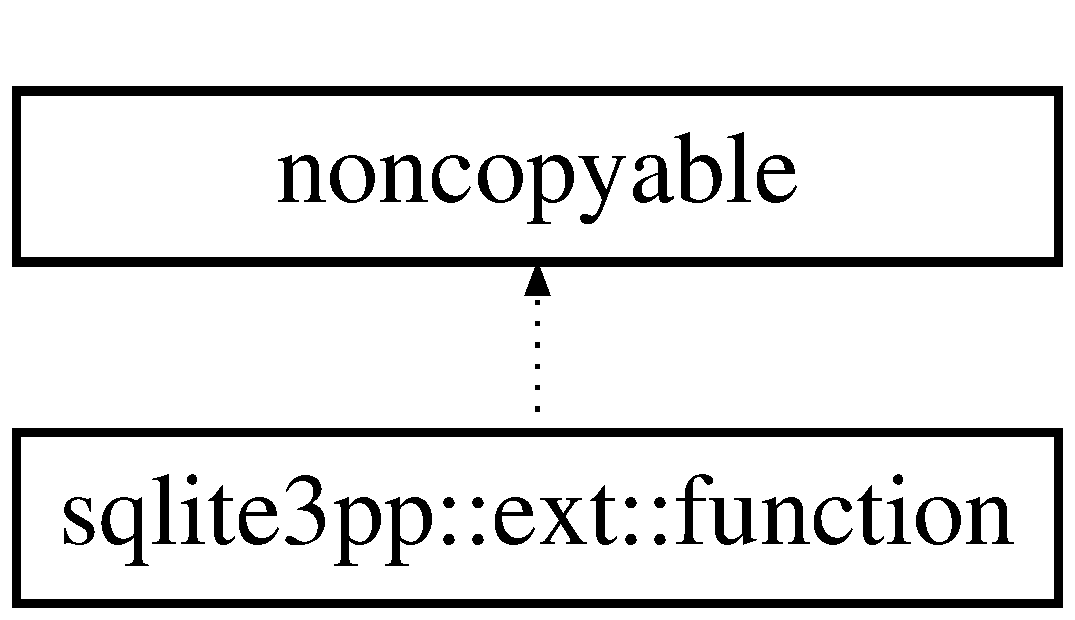
\includegraphics[height=2.000000cm]{classsqlite3pp_1_1ext_1_1function}
\end{center}
\end{figure}
\subsection*{Public Types}
\begin{DoxyCompactItemize}
\item 
\hypertarget{classsqlite3pp_1_1ext_1_1function_a2bcae882e1f5154bc37e8bea893a7442}{typedef boost\-::function$<$ void(\hyperlink{classsqlite3pp_1_1ext_1_1context}{context} \&)$>$ {\bfseries function\-\_\-handler}}\label{classsqlite3pp_1_1ext_1_1function_a2bcae882e1f5154bc37e8bea893a7442}

\item 
\hypertarget{classsqlite3pp_1_1ext_1_1function_a0518a4144a7080bbf79ec7c84dfebcb1}{typedef boost\-::shared\-\_\-ptr\\*
$<$ boost\-::function\-\_\-base $>$ {\bfseries pfunction\-\_\-base}}\label{classsqlite3pp_1_1ext_1_1function_a0518a4144a7080bbf79ec7c84dfebcb1}

\end{DoxyCompactItemize}
\subsection*{Public Member Functions}
\begin{DoxyCompactItemize}
\item 
\hypertarget{classsqlite3pp_1_1ext_1_1function_ac4dce0f916f9f83366794d4124877044}{{\bfseries function} (\hyperlink{classsqlite3pp_1_1database}{database} \&db)}\label{classsqlite3pp_1_1ext_1_1function_ac4dce0f916f9f83366794d4124877044}

\item 
\hypertarget{classsqlite3pp_1_1ext_1_1function_ab01204cf5560b17a72830d48bbe0cbfe}{int {\bfseries create} (char const $\ast$name, function\-\_\-handler h, int nargs=0)}\label{classsqlite3pp_1_1ext_1_1function_ab01204cf5560b17a72830d48bbe0cbfe}

\item 
\hypertarget{classsqlite3pp_1_1ext_1_1function_add028483ddbb6bdd8a972099116b0bca}{{\footnotesize template$<$class F $>$ }\\int {\bfseries create} (char const $\ast$name, boost\-::function$<$ F $>$ h)}\label{classsqlite3pp_1_1ext_1_1function_add028483ddbb6bdd8a972099116b0bca}

\end{DoxyCompactItemize}


The documentation for this class was generated from the following files\-:\begin{DoxyCompactItemize}
\item 
sqlite3ppext.\-h\item 
sqlite3ppext.\-cpp\end{DoxyCompactItemize}

\hypertarget{classsqlite3pp_1_1query_1_1rows_1_1getstream}{\section{sqlite3pp\-:\-:query\-:\-:rows\-:\-:getstream Class Reference}
\label{classsqlite3pp_1_1query_1_1rows_1_1getstream}\index{sqlite3pp\-::query\-::rows\-::getstream@{sqlite3pp\-::query\-::rows\-::getstream}}
}
\subsection*{Public Member Functions}
\begin{DoxyCompactItemize}
\item 
\hypertarget{classsqlite3pp_1_1query_1_1rows_1_1getstream_ae8b0fae73fa51d56bf1a103b9b483199}{{\bfseries getstream} (\hyperlink{classsqlite3pp_1_1query_1_1rows}{rows} $\ast$rws, int idx)}\label{classsqlite3pp_1_1query_1_1rows_1_1getstream_ae8b0fae73fa51d56bf1a103b9b483199}

\item 
\hypertarget{classsqlite3pp_1_1query_1_1rows_1_1getstream_ad8a1f23166695ebac99f88ff600bf097}{{\footnotesize template$<$class T $>$ }\\\hyperlink{classsqlite3pp_1_1query_1_1rows_1_1getstream}{getstream} \& {\bfseries operator$>$$>$} (T \&value)}\label{classsqlite3pp_1_1query_1_1rows_1_1getstream_ad8a1f23166695ebac99f88ff600bf097}

\end{DoxyCompactItemize}


The documentation for this class was generated from the following files\-:\begin{DoxyCompactItemize}
\item 
sqlite3pp.\-h\item 
sqlite3pp.\-cpp\end{DoxyCompactItemize}

\hypertarget{classsqlite3pp_1_1null__type}{\section{sqlite3pp\-:\-:null\-\_\-type Class Reference}
\label{classsqlite3pp_1_1null__type}\index{sqlite3pp\-::null\-\_\-type@{sqlite3pp\-::null\-\_\-type}}
}


The documentation for this class was generated from the following file\-:\begin{DoxyCompactItemize}
\item 
sqlite3pp.\-h\end{DoxyCompactItemize}

\hypertarget{classsqlite3pp_1_1query}{\section{sqlite3pp\-:\-:query Class Reference}
\label{classsqlite3pp_1_1query}\index{sqlite3pp\-::query@{sqlite3pp\-::query}}
}
Inheritance diagram for sqlite3pp\-:\-:query\-:\begin{figure}[H]
\begin{center}
\leavevmode
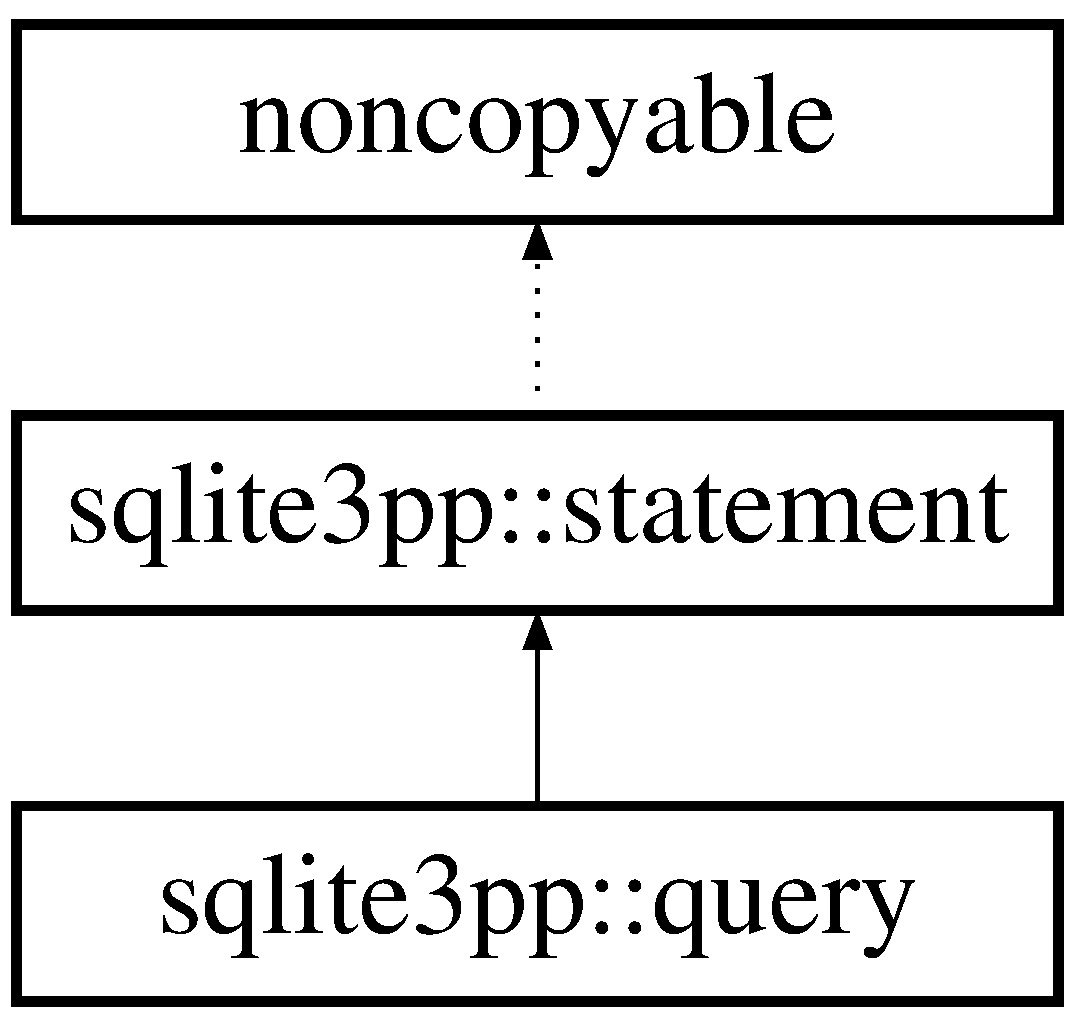
\includegraphics[height=3.000000cm]{classsqlite3pp_1_1query}
\end{center}
\end{figure}
\subsection*{Classes}
\begin{DoxyCompactItemize}
\item 
class \hyperlink{classsqlite3pp_1_1query_1_1query__iterator}{query\-\_\-iterator}
\item 
class \hyperlink{classsqlite3pp_1_1query_1_1rows}{rows}
\end{DoxyCompactItemize}
\subsection*{Public Types}
\begin{DoxyCompactItemize}
\item 
\hypertarget{classsqlite3pp_1_1query_a8a8af0cf5d5750fe6b3579fcd37d3c43}{typedef \hyperlink{classsqlite3pp_1_1query_1_1query__iterator}{query\-\_\-iterator} {\bfseries iterator}}\label{classsqlite3pp_1_1query_a8a8af0cf5d5750fe6b3579fcd37d3c43}

\end{DoxyCompactItemize}
\subsection*{Public Member Functions}
\begin{DoxyCompactItemize}
\item 
\hypertarget{classsqlite3pp_1_1query_ae8401752284f0855debd91c435f13fb3}{{\bfseries query} (\hyperlink{classsqlite3pp_1_1database}{database} \&db, char const $\ast$stmt=0)}\label{classsqlite3pp_1_1query_ae8401752284f0855debd91c435f13fb3}

\item 
\hypertarget{classsqlite3pp_1_1query_a174cfff81897580685ff999d498fb459}{int {\bfseries column\-\_\-count} () const }\label{classsqlite3pp_1_1query_a174cfff81897580685ff999d498fb459}

\item 
\hypertarget{classsqlite3pp_1_1query_ac4aea749613026c3519eafee2189f020}{char const $\ast$ {\bfseries column\-\_\-name} (int idx) const }\label{classsqlite3pp_1_1query_ac4aea749613026c3519eafee2189f020}

\item 
\hypertarget{classsqlite3pp_1_1query_ac36113f906c0a9285ceeb900a3a7cbea}{char const $\ast$ {\bfseries column\-\_\-decltype} (int idx) const }\label{classsqlite3pp_1_1query_ac36113f906c0a9285ceeb900a3a7cbea}

\item 
\hypertarget{classsqlite3pp_1_1query_a22b1c6cfc91c5c31d8f0be7a71e2b9e4}{\hyperlink{classsqlite3pp_1_1query_1_1query__iterator}{iterator} {\bfseries begin} ()}\label{classsqlite3pp_1_1query_a22b1c6cfc91c5c31d8f0be7a71e2b9e4}

\item 
\hypertarget{classsqlite3pp_1_1query_a005f2a324a5c2c724cfd0ecf02d618be}{\hyperlink{classsqlite3pp_1_1query_1_1query__iterator}{iterator} {\bfseries end} ()}\label{classsqlite3pp_1_1query_a005f2a324a5c2c724cfd0ecf02d618be}

\end{DoxyCompactItemize}
\subsection*{Additional Inherited Members}


The documentation for this class was generated from the following files\-:\begin{DoxyCompactItemize}
\item 
sqlite3pp.\-h\item 
sqlite3pp.\-cpp\end{DoxyCompactItemize}

\hypertarget{classsqlite3pp_1_1query_1_1query__iterator}{\section{sqlite3pp\-:\-:query\-:\-:query\-\_\-iterator Class Reference}
\label{classsqlite3pp_1_1query_1_1query__iterator}\index{sqlite3pp\-::query\-::query\-\_\-iterator@{sqlite3pp\-::query\-::query\-\_\-iterator}}
}
Inheritance diagram for sqlite3pp\-:\-:query\-:\-:query\-\_\-iterator\-:\begin{figure}[H]
\begin{center}
\leavevmode
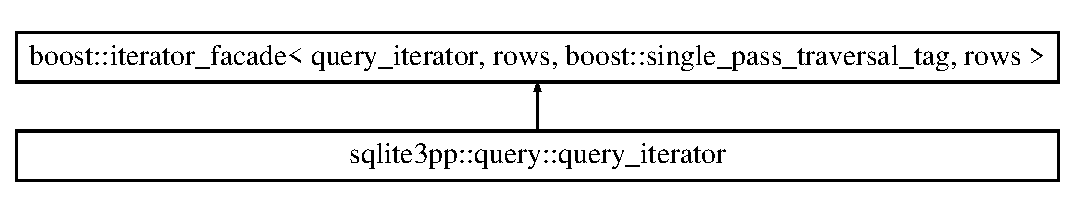
\includegraphics[height=2.000000cm]{classsqlite3pp_1_1query_1_1query__iterator}
\end{center}
\end{figure}
\subsection*{Public Member Functions}
\begin{DoxyCompactItemize}
\item 
\hypertarget{classsqlite3pp_1_1query_1_1query__iterator_a1b1a753061b77cfb060190cf6ea4562f}{{\bfseries query\-\_\-iterator} (\hyperlink{classsqlite3pp_1_1query}{query} $\ast$cmd)}\label{classsqlite3pp_1_1query_1_1query__iterator_a1b1a753061b77cfb060190cf6ea4562f}

\end{DoxyCompactItemize}
\subsection*{Friends}
\begin{DoxyCompactItemize}
\item 
\hypertarget{classsqlite3pp_1_1query_1_1query__iterator_ac09f73e325921cc50ebcd96bed0f8096}{class {\bfseries boost\-::iterator\-\_\-core\-\_\-access}}\label{classsqlite3pp_1_1query_1_1query__iterator_ac09f73e325921cc50ebcd96bed0f8096}

\end{DoxyCompactItemize}


The documentation for this class was generated from the following files\-:\begin{DoxyCompactItemize}
\item 
sqlite3pp.\-h\item 
sqlite3pp.\-cpp\end{DoxyCompactItemize}

\hypertarget{classsqlite3pp_1_1query_1_1rows}{\section{sqlite3pp\-:\-:query\-:\-:rows Class Reference}
\label{classsqlite3pp_1_1query_1_1rows}\index{sqlite3pp\-::query\-::rows@{sqlite3pp\-::query\-::rows}}
}
\subsection*{Classes}
\begin{DoxyCompactItemize}
\item 
class \hyperlink{classsqlite3pp_1_1query_1_1rows_1_1getstream}{getstream}
\end{DoxyCompactItemize}
\subsection*{Public Member Functions}
\begin{DoxyCompactItemize}
\item 
\hypertarget{classsqlite3pp_1_1query_1_1rows_a0e1a157e8839291cde7ead8ea243b882}{{\bfseries rows} (sqlite3\-\_\-stmt $\ast$stmt)}\label{classsqlite3pp_1_1query_1_1rows_a0e1a157e8839291cde7ead8ea243b882}

\item 
\hypertarget{classsqlite3pp_1_1query_1_1rows_a8564cf19c09033fb3244b91b0d320768}{int {\bfseries data\-\_\-count} () const }\label{classsqlite3pp_1_1query_1_1rows_a8564cf19c09033fb3244b91b0d320768}

\item 
\hypertarget{classsqlite3pp_1_1query_1_1rows_abd3bd9f1f490ad38b5adef4f84135201}{int {\bfseries column\-\_\-type} (int idx) const }\label{classsqlite3pp_1_1query_1_1rows_abd3bd9f1f490ad38b5adef4f84135201}

\item 
\hypertarget{classsqlite3pp_1_1query_1_1rows_a17881e50948d6c16941ddab08f2479f7}{int {\bfseries column\-\_\-bytes} (int idx) const }\label{classsqlite3pp_1_1query_1_1rows_a17881e50948d6c16941ddab08f2479f7}

\item 
\hypertarget{classsqlite3pp_1_1query_1_1rows_af25a44d5d184d65cf2a6a8f60069acb9}{{\footnotesize template$<$class T $>$ }\\T {\bfseries get} (int idx) const }\label{classsqlite3pp_1_1query_1_1rows_af25a44d5d184d65cf2a6a8f60069acb9}

\item 
\hypertarget{classsqlite3pp_1_1query_1_1rows_a40739dfe3bc4622629bbd5efbcd4a039}{{\footnotesize template$<$class T1 $>$ }\\boost\-::tuple$<$ T1 $>$ {\bfseries get\-\_\-columns} (int idx1) const }\label{classsqlite3pp_1_1query_1_1rows_a40739dfe3bc4622629bbd5efbcd4a039}

\item 
\hypertarget{classsqlite3pp_1_1query_1_1rows_a0db39c837c4089eb16a4149f271ecab3}{{\footnotesize template$<$class T1 , class T2 $>$ }\\boost\-::tuple$<$ T1, T2 $>$ {\bfseries get\-\_\-columns} (int idx1, int idx2) const }\label{classsqlite3pp_1_1query_1_1rows_a0db39c837c4089eb16a4149f271ecab3}

\item 
\hypertarget{classsqlite3pp_1_1query_1_1rows_a10758ebf6d4711ca3cdbc2d10cdfc079}{{\footnotesize template$<$class T1 , class T2 , class T3 $>$ }\\boost\-::tuple$<$ T1, T2, T3 $>$ {\bfseries get\-\_\-columns} (int idx1, int idx2, int idx3) const }\label{classsqlite3pp_1_1query_1_1rows_a10758ebf6d4711ca3cdbc2d10cdfc079}

\item 
\hypertarget{classsqlite3pp_1_1query_1_1rows_aacde59252afbe52db88a3705f9c2a1ca}{{\footnotesize template$<$class T1 , class T2 , class T3 , class T4 $>$ }\\boost\-::tuple$<$ T1, T2, T3, T4 $>$ {\bfseries get\-\_\-columns} (int idx1, int idx2, int idx3, int idx4) const }\label{classsqlite3pp_1_1query_1_1rows_aacde59252afbe52db88a3705f9c2a1ca}

\item 
\hypertarget{classsqlite3pp_1_1query_1_1rows_ab5b41378853b226af9232d795c29d914}{{\footnotesize template$<$class T1 , class T2 , class T3 , class T4 , class T5 $>$ }\\boost\-::tuple$<$ T1, T2, T3, T4, T5 $>$ {\bfseries get\-\_\-columns} (int idx1, int idx2, int idx3, int idx4, int idx5) const }\label{classsqlite3pp_1_1query_1_1rows_ab5b41378853b226af9232d795c29d914}

\item 
\hypertarget{classsqlite3pp_1_1query_1_1rows_aa8cbb31728dc1140b61fa5223f47c1e7}{{\footnotesize template$<$class T1 , class T2 , class T3 , class T4 , class T5 , class T6 $>$ }\\boost\-::tuple$<$ T1, T2, T3, T4, \\*
T5, T6 $>$ {\bfseries get\-\_\-columns} (int idx1, int idx2, int idx3, int idx4, int idx5, int idx6) const }\label{classsqlite3pp_1_1query_1_1rows_aa8cbb31728dc1140b61fa5223f47c1e7}

\item 
\hypertarget{classsqlite3pp_1_1query_1_1rows_a5d8a09258cdaf11a84fa6aba00061c9c}{{\footnotesize template$<$class T1 , class T2 , class T3 , class T4 , class T5 , class T6 , class T7 $>$ }\\boost\-::tuple$<$ T1, T2, T3, T4, \\*
T5, T6, T7 $>$ {\bfseries get\-\_\-columns} (int idx1, int idx2, int idx3, int idx4, int idx5, int idx6, int idx7) const }\label{classsqlite3pp_1_1query_1_1rows_a5d8a09258cdaf11a84fa6aba00061c9c}

\item 
\hypertarget{classsqlite3pp_1_1query_1_1rows_ae2d0a357149b380cb4b756489ea7c285}{{\footnotesize template$<$class T1 , class T2 , class T3 , class T4 , class T5 , class T6 , class T7 , class T8 $>$ }\\boost\-::tuple$<$ T1, T2, T3, T4, \\*
T5, T6, T7, T8 $>$ {\bfseries get\-\_\-columns} (int idx1, int idx2, int idx3, int idx4, int idx5, int idx6, int idx7, int idx8) const }\label{classsqlite3pp_1_1query_1_1rows_ae2d0a357149b380cb4b756489ea7c285}

\item 
\hypertarget{classsqlite3pp_1_1query_1_1rows_a0b3882a05309d4adaa5a87410e82025a}{\hyperlink{classsqlite3pp_1_1query_1_1rows_1_1getstream}{getstream} {\bfseries getter} (int idx=0)}\label{classsqlite3pp_1_1query_1_1rows_a0b3882a05309d4adaa5a87410e82025a}

\end{DoxyCompactItemize}


The documentation for this class was generated from the following files\-:\begin{DoxyCompactItemize}
\item 
sqlite3pp.\-h\item 
sqlite3pp.\-cpp\end{DoxyCompactItemize}

\hypertarget{classsqlite3pp_1_1statement}{\section{sqlite3pp\-:\-:statement Class Reference}
\label{classsqlite3pp_1_1statement}\index{sqlite3pp\-::statement@{sqlite3pp\-::statement}}
}
Inheritance diagram for sqlite3pp\-:\-:statement\-:\begin{figure}[H]
\begin{center}
\leavevmode
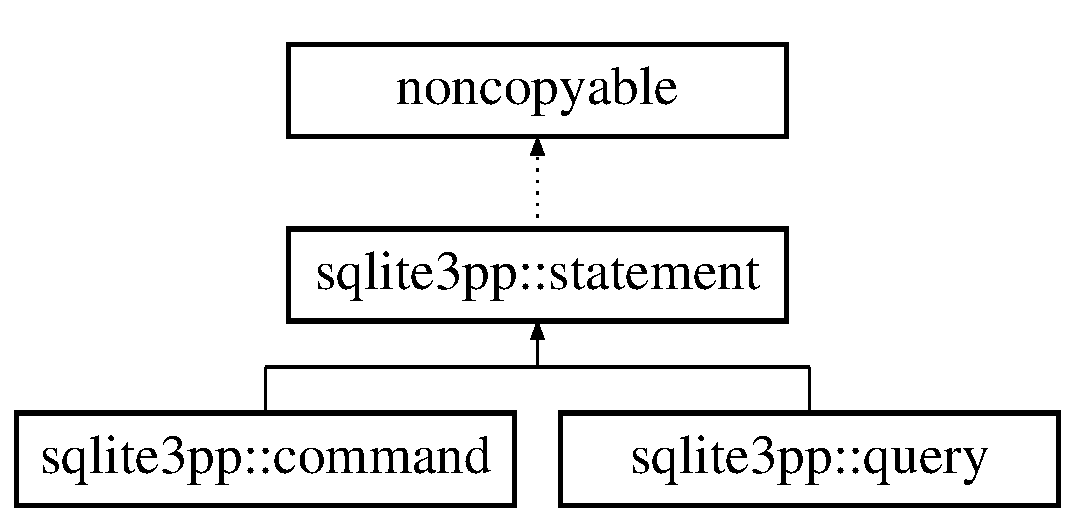
\includegraphics[height=3.000000cm]{classsqlite3pp_1_1statement}
\end{center}
\end{figure}
\subsection*{Public Member Functions}
\begin{DoxyCompactItemize}
\item 
\hypertarget{classsqlite3pp_1_1statement_aafcd2e3f9245e56a7beae1ad64215aa7}{int {\bfseries prepare} (char const $\ast$stmt)}\label{classsqlite3pp_1_1statement_aafcd2e3f9245e56a7beae1ad64215aa7}

\item 
\hypertarget{classsqlite3pp_1_1statement_a5c8ffdb4c3fda921cd70223496591933}{int {\bfseries finish} ()}\label{classsqlite3pp_1_1statement_a5c8ffdb4c3fda921cd70223496591933}

\item 
\hypertarget{classsqlite3pp_1_1statement_af6671aba58cf79f489212123380b1971}{int {\bfseries bind} (int idx, int value)}\label{classsqlite3pp_1_1statement_af6671aba58cf79f489212123380b1971}

\item 
\hypertarget{classsqlite3pp_1_1statement_a1f56c2c4135b96720d319ffeaeccb4a3}{int {\bfseries bind} (int idx, double value)}\label{classsqlite3pp_1_1statement_a1f56c2c4135b96720d319ffeaeccb4a3}

\item 
\hypertarget{classsqlite3pp_1_1statement_a4a14707c8b72fa2f3d09bc3765a01bfc}{int {\bfseries bind} (int idx, long long int value)}\label{classsqlite3pp_1_1statement_a4a14707c8b72fa2f3d09bc3765a01bfc}

\item 
\hypertarget{classsqlite3pp_1_1statement_a0c02d737b01faeeab329226b9fa9debd}{int {\bfseries bind} (int idx, char const $\ast$value, bool fstatic=true)}\label{classsqlite3pp_1_1statement_a0c02d737b01faeeab329226b9fa9debd}

\item 
\hypertarget{classsqlite3pp_1_1statement_a34025ae792bd02f38221a82dd3b887f3}{int {\bfseries bind} (int idx, void const $\ast$value, int n, bool fstatic=true)}\label{classsqlite3pp_1_1statement_a34025ae792bd02f38221a82dd3b887f3}

\item 
\hypertarget{classsqlite3pp_1_1statement_af980d3c0cb73bcdff105c58a46dc50e3}{int {\bfseries bind} (int idx)}\label{classsqlite3pp_1_1statement_af980d3c0cb73bcdff105c58a46dc50e3}

\item 
\hypertarget{classsqlite3pp_1_1statement_a1a9b9dd56d2b6aada8850e6ad24f2288}{int {\bfseries bind} (int idx, \hyperlink{classsqlite3pp_1_1null__type}{null\-\_\-type})}\label{classsqlite3pp_1_1statement_a1a9b9dd56d2b6aada8850e6ad24f2288}

\item 
\hypertarget{classsqlite3pp_1_1statement_a9cac65a01fdaf5122332dc9e0026c759}{int {\bfseries bind} (char const $\ast$name, int value)}\label{classsqlite3pp_1_1statement_a9cac65a01fdaf5122332dc9e0026c759}

\item 
\hypertarget{classsqlite3pp_1_1statement_a9f1ad83c30d8807131b2276a7f58b884}{int {\bfseries bind} (char const $\ast$name, double value)}\label{classsqlite3pp_1_1statement_a9f1ad83c30d8807131b2276a7f58b884}

\item 
\hypertarget{classsqlite3pp_1_1statement_ad4e4f332f328cb88d711895dc21c1336}{int {\bfseries bind} (char const $\ast$name, long long int value)}\label{classsqlite3pp_1_1statement_ad4e4f332f328cb88d711895dc21c1336}

\item 
\hypertarget{classsqlite3pp_1_1statement_aa7cc4268bac627bf48475ee665fa9ed7}{int {\bfseries bind} (char const $\ast$name, char const $\ast$value, bool fstatic=true)}\label{classsqlite3pp_1_1statement_aa7cc4268bac627bf48475ee665fa9ed7}

\item 
\hypertarget{classsqlite3pp_1_1statement_a21938505af5ed1bf8063e66f4943d7ec}{int {\bfseries bind} (char const $\ast$name, void const $\ast$value, int n, bool fstatic=true)}\label{classsqlite3pp_1_1statement_a21938505af5ed1bf8063e66f4943d7ec}

\item 
\hypertarget{classsqlite3pp_1_1statement_ab651ec3075a43e97fcb0868c896da561}{int {\bfseries bind} (char const $\ast$name)}\label{classsqlite3pp_1_1statement_ab651ec3075a43e97fcb0868c896da561}

\item 
\hypertarget{classsqlite3pp_1_1statement_a27e20f9382766a79229dfe824a7dbd4b}{int {\bfseries bind} (char const $\ast$name, \hyperlink{classsqlite3pp_1_1null__type}{null\-\_\-type})}\label{classsqlite3pp_1_1statement_a27e20f9382766a79229dfe824a7dbd4b}

\item 
\hypertarget{classsqlite3pp_1_1statement_ab895bf77dae14a2854ee58716883d434}{int {\bfseries step} ()}\label{classsqlite3pp_1_1statement_ab895bf77dae14a2854ee58716883d434}

\item 
\hypertarget{classsqlite3pp_1_1statement_a46b99b07c787f688a0857abafa2be72d}{int {\bfseries reset} ()}\label{classsqlite3pp_1_1statement_a46b99b07c787f688a0857abafa2be72d}

\end{DoxyCompactItemize}
\subsection*{Protected Member Functions}
\begin{DoxyCompactItemize}
\item 
\hypertarget{classsqlite3pp_1_1statement_a3f762e8ad30b0eee07202fbf3b96dd6e}{{\bfseries statement} (\hyperlink{classsqlite3pp_1_1database}{database} \&db, char const $\ast$stmt=0)}\label{classsqlite3pp_1_1statement_a3f762e8ad30b0eee07202fbf3b96dd6e}

\item 
\hypertarget{classsqlite3pp_1_1statement_a591d916bd0845327c7c4d9c9449f0ae2}{int {\bfseries prepare\-\_\-impl} (char const $\ast$stmt)}\label{classsqlite3pp_1_1statement_a591d916bd0845327c7c4d9c9449f0ae2}

\item 
\hypertarget{classsqlite3pp_1_1statement_a4fa7407507a5436f523b843663ccb86f}{int {\bfseries finish\-\_\-impl} (sqlite3\-\_\-stmt $\ast$stmt)}\label{classsqlite3pp_1_1statement_a4fa7407507a5436f523b843663ccb86f}

\end{DoxyCompactItemize}
\subsection*{Protected Attributes}
\begin{DoxyCompactItemize}
\item 
\hypertarget{classsqlite3pp_1_1statement_a5f37049058928eb181e8480757b2dbb7}{\hyperlink{classsqlite3pp_1_1database}{database} \& {\bfseries db\-\_\-}}\label{classsqlite3pp_1_1statement_a5f37049058928eb181e8480757b2dbb7}

\item 
\hypertarget{classsqlite3pp_1_1statement_a0bd419a1e5f45de676eb2c4a5e4d4f3d}{sqlite3\-\_\-stmt $\ast$ {\bfseries stmt\-\_\-}}\label{classsqlite3pp_1_1statement_a0bd419a1e5f45de676eb2c4a5e4d4f3d}

\item 
\hypertarget{classsqlite3pp_1_1statement_a1adff22d514901074aab555dce882881}{char const $\ast$ {\bfseries tail\-\_\-}}\label{classsqlite3pp_1_1statement_a1adff22d514901074aab555dce882881}

\end{DoxyCompactItemize}


The documentation for this class was generated from the following files\-:\begin{DoxyCompactItemize}
\item 
sqlite3pp.\-h\item 
sqlite3pp.\-cpp\end{DoxyCompactItemize}

\hypertarget{class_texto}{\section{Texto Class Reference}
\label{class_texto}\index{Texto@{Texto}}
}


\hyperlink{class_texto}{Texto} /abstract/ class.  




{\ttfamily \#include $<$Texto.\-h$>$}



Inheritance diagram for Texto\-:
\nopagebreak
\begin{figure}[H]
\begin{center}
\leavevmode
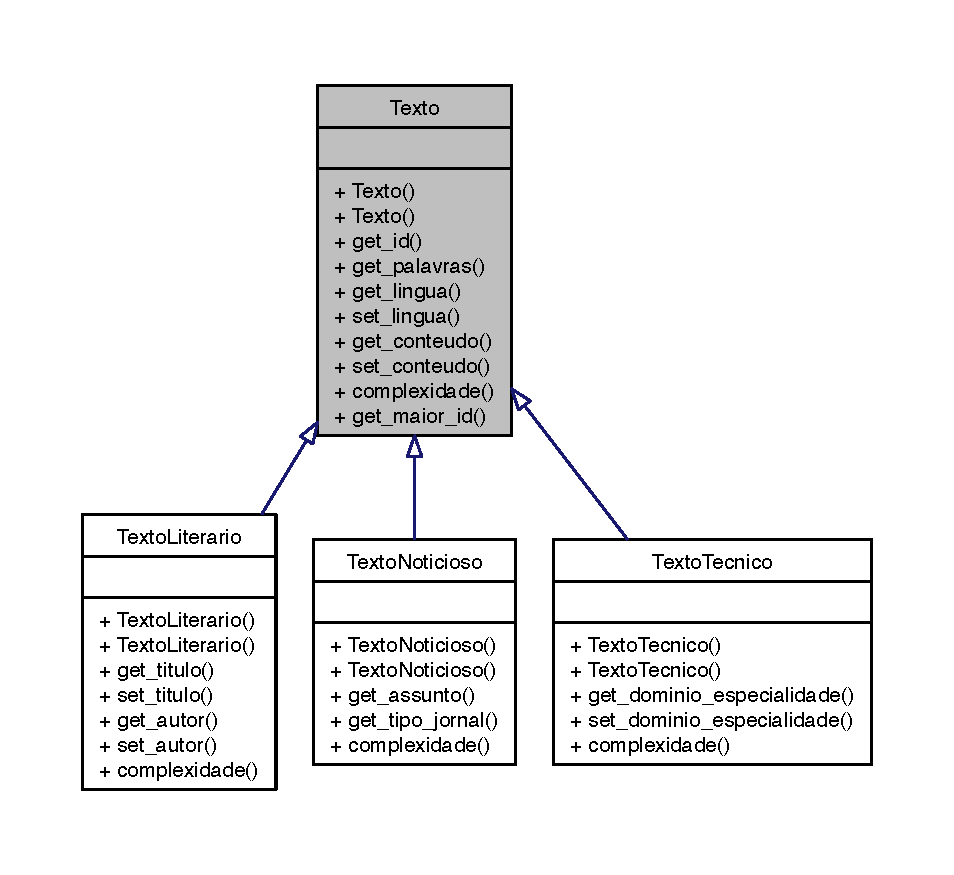
\includegraphics[width=350pt]{class_texto__inherit__graph}
\end{center}
\end{figure}


Collaboration diagram for Texto\-:
\nopagebreak
\begin{figure}[H]
\begin{center}
\leavevmode
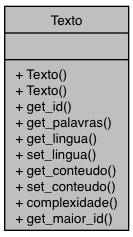
\includegraphics[width=172pt]{class_texto__coll__graph}
\end{center}
\end{figure}
\subsection*{Public Member Functions}
\begin{DoxyCompactItemize}
\item 
\hyperlink{class_texto_a7034548c1e8e2007b0825ef3a01b1b88}{Texto} (unsigned int id, std\-::string lingua, std\-::string conteudo)
\begin{DoxyCompactList}\small\item\em Class Constructor. \end{DoxyCompactList}\item 
\hyperlink{class_texto_a3ccc9eb8eb980eda5e5f6583cbb60425}{Texto} (unsigned int id, std\-::string lingua, unsigned long palavras, std\-::string conteudo)
\begin{DoxyCompactList}\small\item\em Class Constructor. \end{DoxyCompactList}\item 
unsigned int \hyperlink{class_texto_a4e1b7a020c3b1cffe4518937cdd6f565}{get\-\_\-id} ()
\begin{DoxyCompactList}\small\item\em Getter for the I\-D of the text. \end{DoxyCompactList}\item 
unsigned long \hyperlink{class_texto_a35e3a0a47350f735a2e46380eafde1e0}{get\-\_\-palavras} () const 
\begin{DoxyCompactList}\small\item\em Getter for the word count of the text content. \end{DoxyCompactList}\item 
std\-::string \hyperlink{class_texto_adfaca963b37bef9a739def84e2c810b6}{get\-\_\-lingua} ()
\begin{DoxyCompactList}\small\item\em Getter for the language of the text. \end{DoxyCompactList}\item 
void \hyperlink{class_texto_a297021cc2780c0bf398119bf0e4977e0}{set\-\_\-lingua} (std\-::string lingua)
\begin{DoxyCompactList}\small\item\em Setter for the language of the text. \end{DoxyCompactList}\item 
std\-::string \hyperlink{class_texto_a01a9590011195b1a258e2d3bd247ceb0}{get\-\_\-conteudo} ()
\begin{DoxyCompactList}\small\item\em Getter for the text content. \end{DoxyCompactList}\item 
void \hyperlink{class_texto_a94ae33fe47a0ef32a5761a12e097910d}{set\-\_\-conteudo} (std\-::string conteudo)
\begin{DoxyCompactList}\small\item\em Setter for the text content. \end{DoxyCompactList}\item 
virtual unsigned int \hyperlink{class_texto_a92e0fb258179999bc6df2a9da1713a1d}{complexidade} ()=0
\begin{DoxyCompactList}\small\item\em Calculates the complexity of the text. \end{DoxyCompactList}\end{DoxyCompactItemize}
\subsection*{Static Public Member Functions}
\begin{DoxyCompactItemize}
\item 
static unsigned int \hyperlink{class_texto_a674eed23fb437d4f07634f9d6559d325}{get\-\_\-maior\-\_\-id} ()
\begin{DoxyCompactList}\small\item\em Getter for the biggest I\-D of the known text objects. \end{DoxyCompactList}\end{DoxyCompactItemize}


\subsection{Detailed Description}
\hyperlink{class_texto}{Texto} /abstract/ class. 

You should not (alas, can not, most compilers won't even allow it) use this class directly. Please use one of the subclasses (\hyperlink{class_texto_tecnico}{Texto\-Tecnico}, \hyperlink{class_texto_literario}{Texto\-Literario} or \hyperlink{class_texto_noticioso}{Texto\-Noticioso}). 

\subsection{Constructor \& Destructor Documentation}
\hypertarget{class_texto_a7034548c1e8e2007b0825ef3a01b1b88}{\index{Texto@{Texto}!Texto@{Texto}}
\index{Texto@{Texto}!Texto@{Texto}}
\subsubsection[{Texto}]{\setlength{\rightskip}{0pt plus 5cm}Texto\-::\-Texto (
\begin{DoxyParamCaption}
\item[{unsigned int}]{id, }
\item[{std\-::string}]{lingua, }
\item[{std\-::string}]{conteudo}
\end{DoxyParamCaption}
)}}\label{class_texto_a7034548c1e8e2007b0825ef3a01b1b88}


Class Constructor. 


\begin{DoxyParams}{Parameters}
{\em id} & The object I\-D. \\
\hline
{\em lingua} & The language the text is written in. \\
\hline
{\em conteudo} & The plain text contents of the text. \\
\hline
\end{DoxyParams}
\hypertarget{class_texto_a3ccc9eb8eb980eda5e5f6583cbb60425}{\index{Texto@{Texto}!Texto@{Texto}}
\index{Texto@{Texto}!Texto@{Texto}}
\subsubsection[{Texto}]{\setlength{\rightskip}{0pt plus 5cm}Texto\-::\-Texto (
\begin{DoxyParamCaption}
\item[{unsigned int}]{id, }
\item[{std\-::string}]{lingua, }
\item[{unsigned long}]{palavras, }
\item[{std\-::string}]{conteudo}
\end{DoxyParamCaption}
)}}\label{class_texto_a3ccc9eb8eb980eda5e5f6583cbb60425}


Class Constructor. 


\begin{DoxyParams}{Parameters}
{\em id} & The object I\-D. \\
\hline
{\em lingua} & The language the text is written in. \\
\hline
{\em palavras} & The word count of conteudo. \\
\hline
{\em conteudo} & The plain text contents of the text. \\
\hline
\end{DoxyParams}


\subsection{Member Function Documentation}
\hypertarget{class_texto_a92e0fb258179999bc6df2a9da1713a1d}{\index{Texto@{Texto}!complexidade@{complexidade}}
\index{complexidade@{complexidade}!Texto@{Texto}}
\subsubsection[{complexidade}]{\setlength{\rightskip}{0pt plus 5cm}unsigned int Texto\-::complexidade (
\begin{DoxyParamCaption}
{}
\end{DoxyParamCaption}
)\hspace{0.3cm}{\ttfamily [pure virtual]}}}\label{class_texto_a92e0fb258179999bc6df2a9da1713a1d}


Calculates the complexity of the text. 

\begin{DoxyReturn}{Returns}
Complexity value. 
\end{DoxyReturn}


Implemented in \hyperlink{class_texto_literario_a286c1693b71a45d4d577dcd15871892c}{Texto\-Literario}, \hyperlink{class_texto_noticioso_a1db491d92e2a467d258f0f470f994981}{Texto\-Noticioso}, and \hyperlink{class_texto_tecnico_aeeeff7367e226e4fc0f0d4cdb692e85d}{Texto\-Tecnico}.

\hypertarget{class_texto_a01a9590011195b1a258e2d3bd247ceb0}{\index{Texto@{Texto}!get\-\_\-conteudo@{get\-\_\-conteudo}}
\index{get\-\_\-conteudo@{get\-\_\-conteudo}!Texto@{Texto}}
\subsubsection[{get\-\_\-conteudo}]{\setlength{\rightskip}{0pt plus 5cm}std\-::string Texto\-::get\-\_\-conteudo (
\begin{DoxyParamCaption}
{}
\end{DoxyParamCaption}
)}}\label{class_texto_a01a9590011195b1a258e2d3bd247ceb0}


Getter for the text content. 

\begin{DoxyReturn}{Returns}
Text Content (in plain text). 
\end{DoxyReturn}
\hypertarget{class_texto_a4e1b7a020c3b1cffe4518937cdd6f565}{\index{Texto@{Texto}!get\-\_\-id@{get\-\_\-id}}
\index{get\-\_\-id@{get\-\_\-id}!Texto@{Texto}}
\subsubsection[{get\-\_\-id}]{\setlength{\rightskip}{0pt plus 5cm}unsigned int Texto\-::get\-\_\-id (
\begin{DoxyParamCaption}
{}
\end{DoxyParamCaption}
)}}\label{class_texto_a4e1b7a020c3b1cffe4518937cdd6f565}


Getter for the I\-D of the text. 

\begin{DoxyReturn}{Returns}
The I\-D. 
\end{DoxyReturn}
\hypertarget{class_texto_adfaca963b37bef9a739def84e2c810b6}{\index{Texto@{Texto}!get\-\_\-lingua@{get\-\_\-lingua}}
\index{get\-\_\-lingua@{get\-\_\-lingua}!Texto@{Texto}}
\subsubsection[{get\-\_\-lingua}]{\setlength{\rightskip}{0pt plus 5cm}std\-::string Texto\-::get\-\_\-lingua (
\begin{DoxyParamCaption}
{}
\end{DoxyParamCaption}
)}}\label{class_texto_adfaca963b37bef9a739def84e2c810b6}


Getter for the language of the text. 

\begin{DoxyReturn}{Returns}
Language of the text. 
\end{DoxyReturn}
\hypertarget{class_texto_a674eed23fb437d4f07634f9d6559d325}{\index{Texto@{Texto}!get\-\_\-maior\-\_\-id@{get\-\_\-maior\-\_\-id}}
\index{get\-\_\-maior\-\_\-id@{get\-\_\-maior\-\_\-id}!Texto@{Texto}}
\subsubsection[{get\-\_\-maior\-\_\-id}]{\setlength{\rightskip}{0pt plus 5cm}unsigned int Texto\-::get\-\_\-maior\-\_\-id (
\begin{DoxyParamCaption}
{}
\end{DoxyParamCaption}
)\hspace{0.3cm}{\ttfamily [static]}}}\label{class_texto_a674eed23fb437d4f07634f9d6559d325}


Getter for the biggest I\-D of the known text objects. 

\begin{DoxyReturn}{Returns}
The biggest known I\-D. 
\end{DoxyReturn}
\hypertarget{class_texto_a35e3a0a47350f735a2e46380eafde1e0}{\index{Texto@{Texto}!get\-\_\-palavras@{get\-\_\-palavras}}
\index{get\-\_\-palavras@{get\-\_\-palavras}!Texto@{Texto}}
\subsubsection[{get\-\_\-palavras}]{\setlength{\rightskip}{0pt plus 5cm}unsigned long Texto\-::get\-\_\-palavras (
\begin{DoxyParamCaption}
{}
\end{DoxyParamCaption}
) const}}\label{class_texto_a35e3a0a47350f735a2e46380eafde1e0}


Getter for the word count of the text content. 

\begin{DoxyReturn}{Returns}
Word Count of the text content. 
\end{DoxyReturn}
\hypertarget{class_texto_a94ae33fe47a0ef32a5761a12e097910d}{\index{Texto@{Texto}!set\-\_\-conteudo@{set\-\_\-conteudo}}
\index{set\-\_\-conteudo@{set\-\_\-conteudo}!Texto@{Texto}}
\subsubsection[{set\-\_\-conteudo}]{\setlength{\rightskip}{0pt plus 5cm}void Texto\-::set\-\_\-conteudo (
\begin{DoxyParamCaption}
\item[{std\-::string}]{conteudo}
\end{DoxyParamCaption}
)}}\label{class_texto_a94ae33fe47a0ef32a5761a12e097910d}


Setter for the text content. 

\begin{DoxyReturn}{Returns}
Text Content (in plain text). 
\end{DoxyReturn}
\hypertarget{class_texto_a297021cc2780c0bf398119bf0e4977e0}{\index{Texto@{Texto}!set\-\_\-lingua@{set\-\_\-lingua}}
\index{set\-\_\-lingua@{set\-\_\-lingua}!Texto@{Texto}}
\subsubsection[{set\-\_\-lingua}]{\setlength{\rightskip}{0pt plus 5cm}void Texto\-::set\-\_\-lingua (
\begin{DoxyParamCaption}
\item[{std\-::string}]{lingua}
\end{DoxyParamCaption}
)}}\label{class_texto_a297021cc2780c0bf398119bf0e4977e0}


Setter for the language of the text. 


\begin{DoxyParams}{Parameters}
{\em lingua} & Language of the text. \\
\hline
\end{DoxyParams}


The documentation for this class was generated from the following files\-:\begin{DoxyCompactItemize}
\item 
\hyperlink{_texto_8h}{Texto.\-h}\item 
\hyperlink{_texto_8cpp}{Texto.\-cpp}\end{DoxyCompactItemize}

\hypertarget{class_texto_literario}{\section{Texto\-Literario Class Reference}
\label{class_texto_literario}\index{Texto\-Literario@{Texto\-Literario}}
}


\hyperlink{class_texto}{Texto} Literario class.  




{\ttfamily \#include $<$Texto\-Literario.\-h$>$}



Inheritance diagram for Texto\-Literario\-:
\nopagebreak
\begin{figure}[H]
\begin{center}
\leavevmode
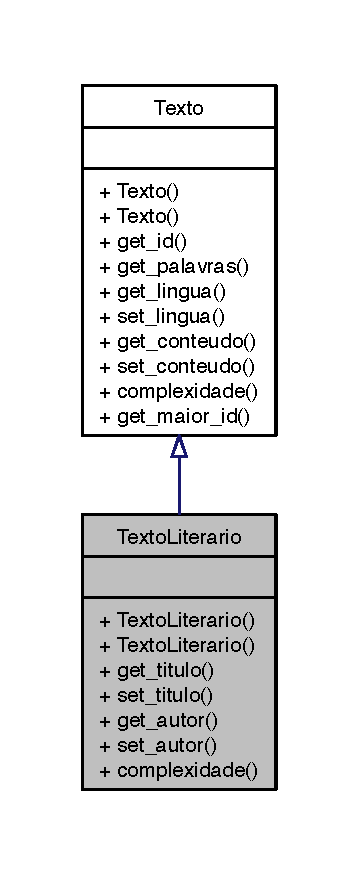
\includegraphics[width=172pt]{class_texto_literario__inherit__graph}
\end{center}
\end{figure}


Collaboration diagram for Texto\-Literario\-:
\nopagebreak
\begin{figure}[H]
\begin{center}
\leavevmode
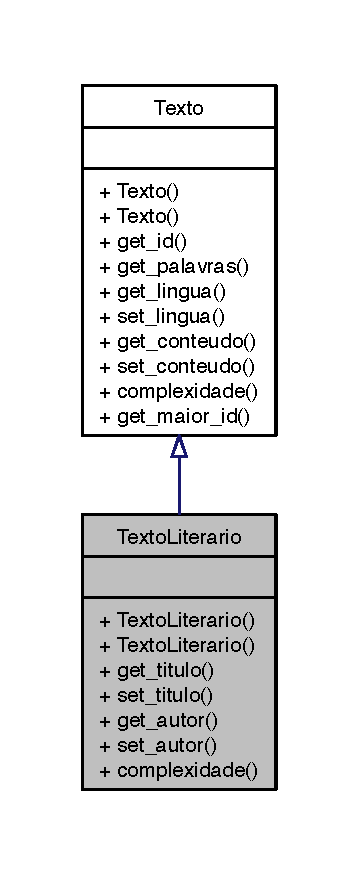
\includegraphics[width=172pt]{class_texto_literario__coll__graph}
\end{center}
\end{figure}
\subsection*{Public Member Functions}
\begin{DoxyCompactItemize}
\item 
\hyperlink{class_texto_literario_addeb2b30770693455c5395a4a3fb941c}{Texto\-Literario} (unsigned int id, std\-::string lingua, std\-::string conteudo, std\-::string titulo, std\-::string autor)
\begin{DoxyCompactList}\small\item\em Class Constructor. \end{DoxyCompactList}\item 
\hyperlink{class_texto_literario_ac8484056631c263a653243b80065114b}{Texto\-Literario} (unsigned int id, std\-::string lingua, unsigned long palavras, std\-::string conteudo, std\-::string titulo, std\-::string autor)
\begin{DoxyCompactList}\small\item\em Class Constructor. \end{DoxyCompactList}\item 
std\-::string \hyperlink{class_texto_literario_adca504c785afdb9e77542b2bdca90a37}{get\-\_\-titulo} ()
\begin{DoxyCompactList}\small\item\em Getter for the title of the text. \end{DoxyCompactList}\item 
void \hyperlink{class_texto_literario_acfb7945b3d45250c316a3b6dc688383c}{set\-\_\-titulo} (std\-::string titulo)
\begin{DoxyCompactList}\small\item\em Setter for the title of the text. \end{DoxyCompactList}\item 
std\-::string \hyperlink{class_texto_literario_acb31c6be6750cea439dde8636bf960ff}{get\-\_\-autor} ()
\begin{DoxyCompactList}\small\item\em Getter for the author of the text. \end{DoxyCompactList}\item 
void \hyperlink{class_texto_literario_a859bcc3c015ebcced7b4691990d3ec2a}{set\-\_\-autor} (std\-::string autor)
\begin{DoxyCompactList}\small\item\em Setter for the author of the text. \end{DoxyCompactList}\item 
unsigned int \hyperlink{class_texto_literario_a286c1693b71a45d4d577dcd15871892c}{complexidade} ()
\begin{DoxyCompactList}\small\item\em Calculates the complexity of the text. \end{DoxyCompactList}\end{DoxyCompactItemize}
\subsection*{Additional Inherited Members}


\subsection{Detailed Description}
\hyperlink{class_texto}{Texto} Literario class. 

Subclass of \hyperlink{class_texto}{Texto}, this handles a specific type of Text (Literary Text). 

\subsection{Constructor \& Destructor Documentation}
\hypertarget{class_texto_literario_addeb2b30770693455c5395a4a3fb941c}{\index{Texto\-Literario@{Texto\-Literario}!Texto\-Literario@{Texto\-Literario}}
\index{Texto\-Literario@{Texto\-Literario}!TextoLiterario@{Texto\-Literario}}
\subsubsection[{Texto\-Literario}]{\setlength{\rightskip}{0pt plus 5cm}Texto\-Literario\-::\-Texto\-Literario (
\begin{DoxyParamCaption}
\item[{unsigned int}]{id, }
\item[{std\-::string}]{lingua, }
\item[{std\-::string}]{conteudo, }
\item[{std\-::string}]{titulo, }
\item[{std\-::string}]{autor}
\end{DoxyParamCaption}
)}}\label{class_texto_literario_addeb2b30770693455c5395a4a3fb941c}


Class Constructor. 


\begin{DoxyParams}{Parameters}
{\em id} & The object I\-D. \\
\hline
{\em lingua} & The language the text is written in. \\
\hline
{\em conteudo} & The plain text contents of the text. \\
\hline
{\em titulo} & The title of the text. \\
\hline
{\em autor} & The author of the text. \\
\hline
\end{DoxyParams}
\hypertarget{class_texto_literario_ac8484056631c263a653243b80065114b}{\index{Texto\-Literario@{Texto\-Literario}!Texto\-Literario@{Texto\-Literario}}
\index{Texto\-Literario@{Texto\-Literario}!TextoLiterario@{Texto\-Literario}}
\subsubsection[{Texto\-Literario}]{\setlength{\rightskip}{0pt plus 5cm}Texto\-Literario\-::\-Texto\-Literario (
\begin{DoxyParamCaption}
\item[{unsigned int}]{id, }
\item[{std\-::string}]{lingua, }
\item[{unsigned long}]{palavras, }
\item[{std\-::string}]{conteudo, }
\item[{std\-::string}]{titulo, }
\item[{std\-::string}]{autor}
\end{DoxyParamCaption}
)}}\label{class_texto_literario_ac8484056631c263a653243b80065114b}


Class Constructor. 


\begin{DoxyParams}{Parameters}
{\em id} & The object I\-D. \\
\hline
{\em lingua} & The language the text is written in. \\
\hline
{\em palavras} & The word coint of conteudo. \\
\hline
{\em conteudo} & The plain text contents of the text. \\
\hline
{\em titulo} & The title of the text. \\
\hline
{\em autor} & The author of the text. \\
\hline
\end{DoxyParams}


\subsection{Member Function Documentation}
\hypertarget{class_texto_literario_a286c1693b71a45d4d577dcd15871892c}{\index{Texto\-Literario@{Texto\-Literario}!complexidade@{complexidade}}
\index{complexidade@{complexidade}!TextoLiterario@{Texto\-Literario}}
\subsubsection[{complexidade}]{\setlength{\rightskip}{0pt plus 5cm}unsigned int Texto\-Literario\-::complexidade (
\begin{DoxyParamCaption}
{}
\end{DoxyParamCaption}
)\hspace{0.3cm}{\ttfamily [virtual]}}}\label{class_texto_literario_a286c1693b71a45d4d577dcd15871892c}


Calculates the complexity of the text. 

\begin{DoxyReturn}{Returns}
Complexity value. 
\end{DoxyReturn}


Reimplemented from \hyperlink{class_texto_a9b397139df00ed907e1e6a1c29e2429b}{Texto}.

\hypertarget{class_texto_literario_acb31c6be6750cea439dde8636bf960ff}{\index{Texto\-Literario@{Texto\-Literario}!get\-\_\-autor@{get\-\_\-autor}}
\index{get\-\_\-autor@{get\-\_\-autor}!TextoLiterario@{Texto\-Literario}}
\subsubsection[{get\-\_\-autor}]{\setlength{\rightskip}{0pt plus 5cm}std\-::string Texto\-Literario\-::get\-\_\-autor (
\begin{DoxyParamCaption}
{}
\end{DoxyParamCaption}
)}}\label{class_texto_literario_acb31c6be6750cea439dde8636bf960ff}


Getter for the author of the text. 

\begin{DoxyReturn}{Returns}
The author of the text. 
\end{DoxyReturn}
\hypertarget{class_texto_literario_adca504c785afdb9e77542b2bdca90a37}{\index{Texto\-Literario@{Texto\-Literario}!get\-\_\-titulo@{get\-\_\-titulo}}
\index{get\-\_\-titulo@{get\-\_\-titulo}!TextoLiterario@{Texto\-Literario}}
\subsubsection[{get\-\_\-titulo}]{\setlength{\rightskip}{0pt plus 5cm}std\-::string Texto\-Literario\-::get\-\_\-titulo (
\begin{DoxyParamCaption}
{}
\end{DoxyParamCaption}
)}}\label{class_texto_literario_adca504c785afdb9e77542b2bdca90a37}


Getter for the title of the text. 

\begin{DoxyReturn}{Returns}
The title of the text. 
\end{DoxyReturn}
\hypertarget{class_texto_literario_a859bcc3c015ebcced7b4691990d3ec2a}{\index{Texto\-Literario@{Texto\-Literario}!set\-\_\-autor@{set\-\_\-autor}}
\index{set\-\_\-autor@{set\-\_\-autor}!TextoLiterario@{Texto\-Literario}}
\subsubsection[{set\-\_\-autor}]{\setlength{\rightskip}{0pt plus 5cm}void Texto\-Literario\-::set\-\_\-autor (
\begin{DoxyParamCaption}
\item[{std\-::string}]{autor}
\end{DoxyParamCaption}
)}}\label{class_texto_literario_a859bcc3c015ebcced7b4691990d3ec2a}


Setter for the author of the text. 

\begin{DoxyReturn}{Returns}
The author of the text. 
\end{DoxyReturn}
\hypertarget{class_texto_literario_acfb7945b3d45250c316a3b6dc688383c}{\index{Texto\-Literario@{Texto\-Literario}!set\-\_\-titulo@{set\-\_\-titulo}}
\index{set\-\_\-titulo@{set\-\_\-titulo}!TextoLiterario@{Texto\-Literario}}
\subsubsection[{set\-\_\-titulo}]{\setlength{\rightskip}{0pt plus 5cm}void Texto\-Literario\-::set\-\_\-titulo (
\begin{DoxyParamCaption}
\item[{std\-::string}]{titulo}
\end{DoxyParamCaption}
)}}\label{class_texto_literario_acfb7945b3d45250c316a3b6dc688383c}


Setter for the title of the text. 

\begin{DoxyReturn}{Returns}
The title of the text. 
\end{DoxyReturn}


The documentation for this class was generated from the following files\-:\begin{DoxyCompactItemize}
\item 
\hyperlink{_texto_literario_8h}{Texto\-Literario.\-h}\item 
\hyperlink{_texto_literario_8cpp}{Texto\-Literario.\-cpp}\end{DoxyCompactItemize}

\hypertarget{class_texto_noticioso}{\section{Texto\-Noticioso Class Reference}
\label{class_texto_noticioso}\index{Texto\-Noticioso@{Texto\-Noticioso}}
}
Inheritance diagram for Texto\-Noticioso\-:\begin{figure}[H]
\begin{center}
\leavevmode
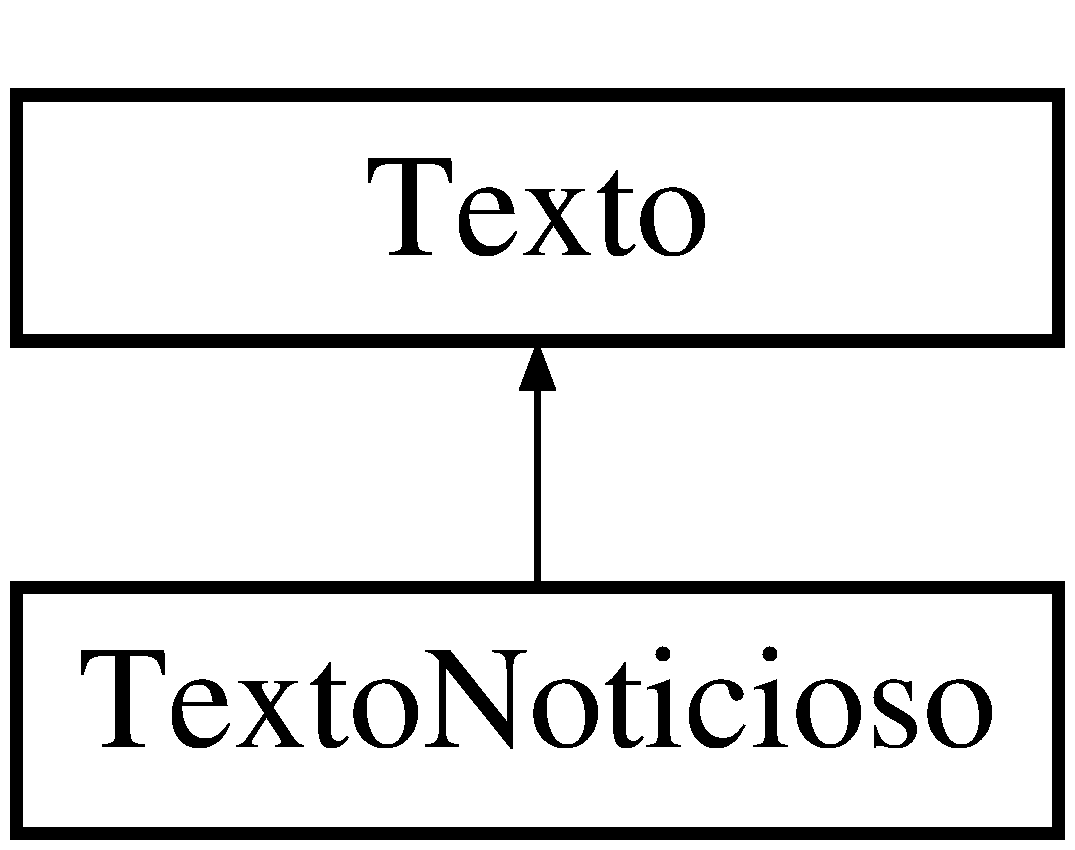
\includegraphics[height=2.000000cm]{class_texto_noticioso}
\end{center}
\end{figure}
\subsection*{Public Member Functions}
\begin{DoxyCompactItemize}
\item 
\hypertarget{class_texto_noticioso_a74a984b14609c5ad38a32cefcc5c9da7}{{\bfseries Texto\-Noticioso} (unsigned int id, std\-::string lingua, std\-::string conteudo, std\-::string assunto, tipo\-\_\-jornal tipo)}\label{class_texto_noticioso_a74a984b14609c5ad38a32cefcc5c9da7}

\item 
\hypertarget{class_texto_noticioso_a9b82b7cd28537c9aa6c214d3439ab6f5}{{\bfseries Texto\-Noticioso} (unsigned int id, std\-::string lingua, unsigned long palavras, std\-::string conteudo, std\-::string assunto, tipo\-\_\-jornal tipo)}\label{class_texto_noticioso_a9b82b7cd28537c9aa6c214d3439ab6f5}

\item 
\hypertarget{class_texto_noticioso_afd686397a10b9e6afa8eb9f1aaf5d21e}{std\-::string {\bfseries get\-\_\-assunto} ()}\label{class_texto_noticioso_afd686397a10b9e6afa8eb9f1aaf5d21e}

\item 
\hypertarget{class_texto_noticioso_ac0edd9121ef61cb4adc360faabecd62b}{tipo\-\_\-jornal {\bfseries get\-\_\-tipo\-\_\-jornal} ()}\label{class_texto_noticioso_ac0edd9121ef61cb4adc360faabecd62b}

\item 
\hypertarget{class_texto_noticioso_a5179276c932815f134aa1e70a6840d64}{unsigned int {\bfseries get\-\_\-complexidade} ()}\label{class_texto_noticioso_a5179276c932815f134aa1e70a6840d64}

\end{DoxyCompactItemize}
\subsection*{Additional Inherited Members}


The documentation for this class was generated from the following files\-:\begin{DoxyCompactItemize}
\item 
Texto\-Noticioso.\-h\item 
Texto\-Noticioso.\-cpp\end{DoxyCompactItemize}

\hypertarget{class_texto_tecnico}{\section{Texto\-Tecnico Class Reference}
\label{class_texto_tecnico}\index{Texto\-Tecnico@{Texto\-Tecnico}}
}


\hyperlink{class_texto}{Texto} Tecnico class.  




{\ttfamily \#include $<$Texto\-Tecnico.\-h$>$}



Inheritance diagram for Texto\-Tecnico\-:
\nopagebreak
\begin{figure}[H]
\begin{center}
\leavevmode
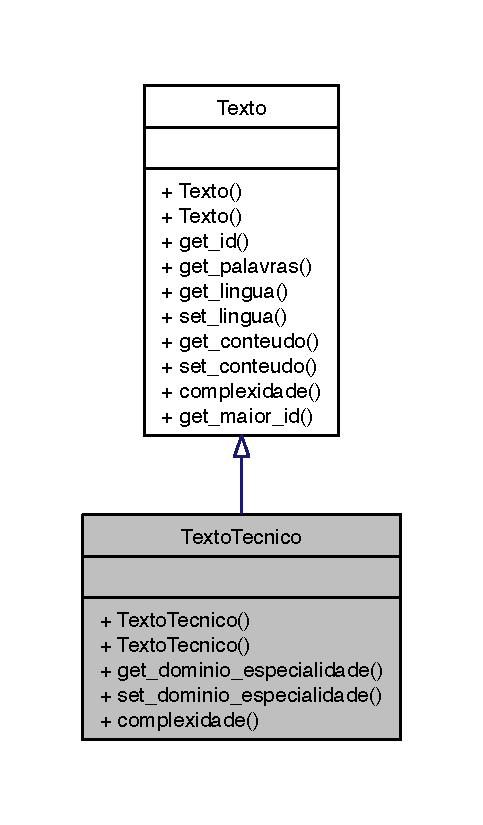
\includegraphics[width=232pt]{class_texto_tecnico__inherit__graph}
\end{center}
\end{figure}
\subsection*{Public Member Functions}
\begin{DoxyCompactItemize}
\item 
\hyperlink{class_texto_tecnico_a4c770469d3a65f750b4551bef18629a9}{Texto\-Tecnico} (unsigned int id, std\-::string lingua, std\-::string conteudo, std\-::string dominio\-\_\-especialidade)
\begin{DoxyCompactList}\small\item\em Class Constructor. \end{DoxyCompactList}\item 
\hyperlink{class_texto_tecnico_adc11a5c4366f90c1f22fc986c4bc2131}{Texto\-Tecnico} (unsigned int id, std\-::string lingua, unsigned long palavras, std\-::string conteudo, std\-::string dominio\-\_\-especialidade)
\begin{DoxyCompactList}\small\item\em Class Constructor. \end{DoxyCompactList}\item 
std\-::string \hyperlink{class_texto_tecnico_af0541bfc3a8fc861eb13abba28a6768d}{get\-\_\-dominio\-\_\-especialidade} ()
\begin{DoxyCompactList}\small\item\em Getter for the text domain. \end{DoxyCompactList}\item 
void \hyperlink{class_texto_tecnico_af66d0b574c0e3316870fb8fdc3223c74}{set\-\_\-dominio\-\_\-especialidade} (std\-::string dominio)
\begin{DoxyCompactList}\small\item\em Setter for the text domain. \end{DoxyCompactList}\item 
unsigned int \hyperlink{class_texto_tecnico_aeeeff7367e226e4fc0f0d4cdb692e85d}{complexidade} ()
\begin{DoxyCompactList}\small\item\em Calculates the complexity of the text. \end{DoxyCompactList}\end{DoxyCompactItemize}
\subsection*{Additional Inherited Members}


\subsection{Detailed Description}
\hyperlink{class_texto}{Texto} Tecnico class. 

Subclass of \hyperlink{class_texto}{Texto}, this handles a specific type of Text (Technical Text). 

\subsection{Constructor \& Destructor Documentation}
\hypertarget{class_texto_tecnico_a4c770469d3a65f750b4551bef18629a9}{\index{Texto\-Tecnico@{Texto\-Tecnico}!Texto\-Tecnico@{Texto\-Tecnico}}
\index{Texto\-Tecnico@{Texto\-Tecnico}!TextoTecnico@{Texto\-Tecnico}}
\subsubsection[{Texto\-Tecnico}]{\setlength{\rightskip}{0pt plus 5cm}Texto\-Tecnico\-::\-Texto\-Tecnico (
\begin{DoxyParamCaption}
\item[{unsigned int}]{id, }
\item[{std\-::string}]{lingua, }
\item[{std\-::string}]{conteudo, }
\item[{std\-::string}]{dominio\-\_\-especialidade}
\end{DoxyParamCaption}
)}}\label{class_texto_tecnico_a4c770469d3a65f750b4551bef18629a9}


Class Constructor. 


\begin{DoxyParams}{Parameters}
{\em id} & The object I\-D. \\
\hline
{\em lingua} & The language the text is written in. \\
\hline
{\em conteudo} & The plain text contents of the text. \\
\hline
{\em dominio\-\_\-especialidade} & The domain of the contents of the text. \\
\hline
\end{DoxyParams}
\hypertarget{class_texto_tecnico_adc11a5c4366f90c1f22fc986c4bc2131}{\index{Texto\-Tecnico@{Texto\-Tecnico}!Texto\-Tecnico@{Texto\-Tecnico}}
\index{Texto\-Tecnico@{Texto\-Tecnico}!TextoTecnico@{Texto\-Tecnico}}
\subsubsection[{Texto\-Tecnico}]{\setlength{\rightskip}{0pt plus 5cm}Texto\-Tecnico\-::\-Texto\-Tecnico (
\begin{DoxyParamCaption}
\item[{unsigned int}]{id, }
\item[{std\-::string}]{lingua, }
\item[{unsigned long}]{palavras, }
\item[{std\-::string}]{conteudo, }
\item[{std\-::string}]{dominio\-\_\-especialidade}
\end{DoxyParamCaption}
)}}\label{class_texto_tecnico_adc11a5c4366f90c1f22fc986c4bc2131}


Class Constructor. 


\begin{DoxyParams}{Parameters}
{\em id} & The object I\-D. \\
\hline
{\em lingua} & The language the text is written in. \\
\hline
{\em palavras} & The word coint of conteudo. \\
\hline
{\em conteudo} & The plain text contents of the text. \\
\hline
{\em dominio\-\_\-especialidade} & The domain of the contents of the text. \\
\hline
\end{DoxyParams}


\subsection{Member Function Documentation}
\hypertarget{class_texto_tecnico_aeeeff7367e226e4fc0f0d4cdb692e85d}{\index{Texto\-Tecnico@{Texto\-Tecnico}!complexidade@{complexidade}}
\index{complexidade@{complexidade}!TextoTecnico@{Texto\-Tecnico}}
\subsubsection[{complexidade}]{\setlength{\rightskip}{0pt plus 5cm}unsigned int Texto\-Tecnico\-::complexidade (
\begin{DoxyParamCaption}
{}
\end{DoxyParamCaption}
)\hspace{0.3cm}{\ttfamily [virtual]}}}\label{class_texto_tecnico_aeeeff7367e226e4fc0f0d4cdb692e85d}


Calculates the complexity of the text. 

\begin{DoxyReturn}{Returns}
Complexity value. 
\end{DoxyReturn}


Reimplemented from \hyperlink{class_texto_a9b397139df00ed907e1e6a1c29e2429b}{Texto}.

\hypertarget{class_texto_tecnico_af0541bfc3a8fc861eb13abba28a6768d}{\index{Texto\-Tecnico@{Texto\-Tecnico}!get\-\_\-dominio\-\_\-especialidade@{get\-\_\-dominio\-\_\-especialidade}}
\index{get\-\_\-dominio\-\_\-especialidade@{get\-\_\-dominio\-\_\-especialidade}!TextoTecnico@{Texto\-Tecnico}}
\subsubsection[{get\-\_\-dominio\-\_\-especialidade}]{\setlength{\rightskip}{0pt plus 5cm}std\-::string Texto\-Tecnico\-::get\-\_\-dominio\-\_\-especialidade (
\begin{DoxyParamCaption}
{}
\end{DoxyParamCaption}
)}}\label{class_texto_tecnico_af0541bfc3a8fc861eb13abba28a6768d}


Getter for the text domain. 

\begin{DoxyReturn}{Returns}
The domain of the text. 
\end{DoxyReturn}
\hypertarget{class_texto_tecnico_af66d0b574c0e3316870fb8fdc3223c74}{\index{Texto\-Tecnico@{Texto\-Tecnico}!set\-\_\-dominio\-\_\-especialidade@{set\-\_\-dominio\-\_\-especialidade}}
\index{set\-\_\-dominio\-\_\-especialidade@{set\-\_\-dominio\-\_\-especialidade}!TextoTecnico@{Texto\-Tecnico}}
\subsubsection[{set\-\_\-dominio\-\_\-especialidade}]{\setlength{\rightskip}{0pt plus 5cm}void Texto\-Tecnico\-::set\-\_\-dominio\-\_\-especialidade (
\begin{DoxyParamCaption}
\item[{std\-::string}]{dominio}
\end{DoxyParamCaption}
)}}\label{class_texto_tecnico_af66d0b574c0e3316870fb8fdc3223c74}


Setter for the text domain. 


\begin{DoxyParams}{Parameters}
{\em dominio} & The domain of the text. \\
\hline
\end{DoxyParams}


The documentation for this class was generated from the following files\-:\begin{DoxyCompactItemize}
\item 
\hyperlink{_texto_tecnico_8h}{Texto\-Tecnico.\-h}\item 
\hyperlink{_texto_tecnico_8cpp}{Texto\-Tecnico.\-cpp}\end{DoxyCompactItemize}

\hypertarget{class_tradutor}{\section{Tradutor Class Reference}
\label{class_tradutor}\index{Tradutor@{Tradutor}}
}


\hyperlink{class_tradutor}{Tradutor} class.  




{\ttfamily \#include $<$Tradutor.\-h$>$}



Collaboration diagram for Tradutor\-:
\nopagebreak
\begin{figure}[H]
\begin{center}
\leavevmode
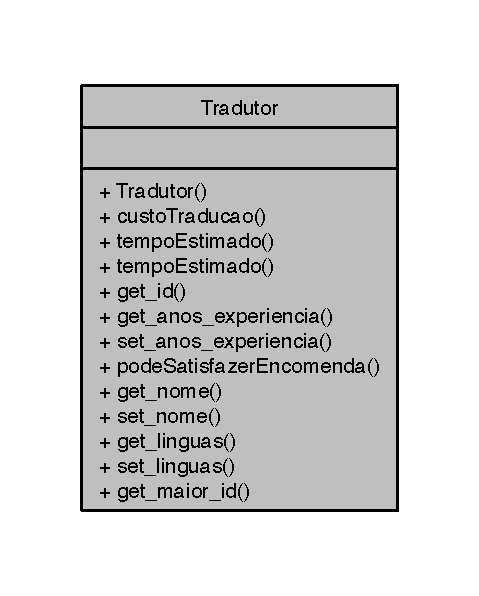
\includegraphics[width=230pt]{class_tradutor__coll__graph}
\end{center}
\end{figure}
\subsection*{Public Member Functions}
\begin{DoxyCompactItemize}
\item 
\hyperlink{class_tradutor_a856f362e6c97ea42d04875e6c9d012e3}{Tradutor} (unsigned int id, std\-::string nome, unsigned int anos\-\_\-experiencia, std\-::vector$<$ std\-::string $>$ linguas)
\begin{DoxyCompactList}\small\item\em Class Constructor. \end{DoxyCompactList}\item 
\hyperlink{class_tradutor_a8b918326e5d4ad49250a87dcab4de424}{Tradutor} (unsigned int id, std\-::string nome, unsigned int anos\-\_\-experiencia, std\-::vector$<$ std\-::string $>$ linguas, bool contratado)
\begin{DoxyCompactList}\small\item\em Class Constructor. \end{DoxyCompactList}\item 
double \hyperlink{class_tradutor_ab55718903fb3e7cc5c1b21b87d64393a}{custo\-Traducao} (\hyperlink{class_texto}{Texto} $\ast$texto)
\begin{DoxyCompactList}\small\item\em Calculates the cost of a given translation. \end{DoxyCompactList}\item 
unsigned int \hyperlink{class_tradutor_a1ca7c608db7e9145e8b9105e19e5900a}{tempo\-Estimado} (\hyperlink{class_texto}{Texto} $\ast$text)
\begin{DoxyCompactList}\small\item\em Calculates the time to fullfill a translation. \end{DoxyCompactList}\item 
unsigned int \hyperlink{class_tradutor_acd53cf00b851be61350100c9aa6ef3c0}{tempo\-Estimado} (\hyperlink{class_encomenda}{Encomenda} $\ast$encomenda)
\begin{DoxyCompactList}\small\item\em Calculates the time to fullfill a given order. \end{DoxyCompactList}\item 
unsigned int \hyperlink{class_tradutor_adc3d4f5ae46ebd92072c644f9fe0e479}{get\-\_\-id} ()
\begin{DoxyCompactList}\small\item\em Getter for the I\-D of the translator. \end{DoxyCompactList}\item 
unsigned int \hyperlink{class_tradutor_a001f11f69661085cb11192d3c6f5d556}{get\-\_\-anos\-\_\-experiencia} ()
\begin{DoxyCompactList}\small\item\em Getter for the years of experience of the translator. \end{DoxyCompactList}\item 
void \hyperlink{class_tradutor_a938cfc1c263b3504fc4d7fbdc939b087}{set\-\_\-anos\-\_\-experiencia} (unsigned int anos\-\_\-exp)
\begin{DoxyCompactList}\small\item\em Setter for the years of experience of the translator. \end{DoxyCompactList}\item 
bool \hyperlink{class_tradutor_a1d22a38c8eaa3753d44b521bb3aab2af}{pode\-Satisfazer\-Encomenda} (\hyperlink{class_encomenda}{Encomenda} $\ast$encomenda)
\begin{DoxyCompactList}\small\item\em Checks if the translator is able to fullfill a given translation. \end{DoxyCompactList}\item 
std\-::string \hyperlink{class_tradutor_aada5c883969bb7903924f2f2ae376026}{get\-\_\-nome} () const 
\begin{DoxyCompactList}\small\item\em Getter for name of the translator. \end{DoxyCompactList}\item 
void \hyperlink{class_tradutor_aa50fdceab0ca03dfe5c2a1639bc5869e}{set\-\_\-nome} (std\-::string nome)
\begin{DoxyCompactList}\small\item\em Setter for name of the translator. \end{DoxyCompactList}\item 
std\-::vector$<$ std\-::string $>$ \hyperlink{class_tradutor_a011b86fa2dae11c6ccdda1cbeb844e94}{get\-\_\-linguas} ()
\begin{DoxyCompactList}\small\item\em Getter for the languages known to the translator. \end{DoxyCompactList}\item 
void \hyperlink{class_tradutor_a83ed5b48e00f3a15c579e209bb01d53f}{set\-\_\-linguas} (std\-::vector$<$ std\-::string $>$ linguas)
\begin{DoxyCompactList}\small\item\em Setter for the languages known to the translator. \end{DoxyCompactList}\item 
bool \hyperlink{class_tradutor_abfd51adb78973d8bbc3bbd35eb5d5b94}{get\-\_\-contratado} ()
\begin{DoxyCompactList}\small\item\em Getter for employment status of the translator. \end{DoxyCompactList}\item 
void \hyperlink{class_tradutor_a00b1ffa1dc1a0eb9fabf6e240a61b94b}{set\-\_\-contratado} (bool cont)
\begin{DoxyCompactList}\small\item\em Setter for employment status of the translator. \end{DoxyCompactList}\item 
bool \hyperlink{class_tradutor_a33f43a54dbef52d8a25796c5ecd6c00a}{operator$<$} (const \hyperlink{class_tradutor}{Tradutor} \&trad) const 
\begin{DoxyCompactList}\small\item\em Overloaded comparision $<$ operator. \end{DoxyCompactList}\end{DoxyCompactItemize}
\subsection*{Static Public Member Functions}
\begin{DoxyCompactItemize}
\item 
static unsigned int \hyperlink{class_tradutor_af2caad7e33c443f238851c5bb2d63930}{get\-\_\-maior\-\_\-id} ()
\begin{DoxyCompactList}\small\item\em Getter for the biggest translator I\-D (of all known translators). \end{DoxyCompactList}\end{DoxyCompactItemize}


\subsection{Detailed Description}
\hyperlink{class_tradutor}{Tradutor} class. 

This class packages the details about a translator and provides some functionality on them. 

\subsection{Constructor \& Destructor Documentation}
\hypertarget{class_tradutor_a856f362e6c97ea42d04875e6c9d012e3}{\index{Tradutor@{Tradutor}!Tradutor@{Tradutor}}
\index{Tradutor@{Tradutor}!Tradutor@{Tradutor}}
\subsubsection[{Tradutor}]{\setlength{\rightskip}{0pt plus 5cm}Tradutor\-::\-Tradutor (
\begin{DoxyParamCaption}
\item[{unsigned int}]{id, }
\item[{std\-::string}]{nome, }
\item[{unsigned int}]{anos\-\_\-experiencia, }
\item[{std\-::vector$<$ std\-::string $>$}]{linguas}
\end{DoxyParamCaption}
)}}\label{class_tradutor_a856f362e6c97ea42d04875e6c9d012e3}


Class Constructor. 


\begin{DoxyParams}{Parameters}
{\em id} & The object I\-D. \\
\hline
{\em nome} & The name of the translator. \\
\hline
{\em anos\-\_\-experiencia} & The experience of the translator, in years. Should be at least 1. \\
\hline
{\em linguas} & The maximum number of days the order should be fullfilled in. \\
\hline
\end{DoxyParams}
\hypertarget{class_tradutor_a8b918326e5d4ad49250a87dcab4de424}{\index{Tradutor@{Tradutor}!Tradutor@{Tradutor}}
\index{Tradutor@{Tradutor}!Tradutor@{Tradutor}}
\subsubsection[{Tradutor}]{\setlength{\rightskip}{0pt plus 5cm}Tradutor\-::\-Tradutor (
\begin{DoxyParamCaption}
\item[{unsigned int}]{id, }
\item[{std\-::string}]{nome, }
\item[{unsigned int}]{anos\-\_\-experiencia, }
\item[{std\-::vector$<$ std\-::string $>$}]{linguas, }
\item[{bool}]{contratado}
\end{DoxyParamCaption}
)}}\label{class_tradutor_a8b918326e5d4ad49250a87dcab4de424}


Class Constructor. 


\begin{DoxyParams}{Parameters}
{\em id} & The object I\-D. \\
\hline
{\em nome} & The name of the translator. \\
\hline
{\em anos\-\_\-experiencia} & The experience of the translator, in years. Should be at least 1. \\
\hline
{\em linguas} & The maximum number of days the order should be fullfilled in. \\
\hline
{\em contratado} & true if the translator is currently hired, false if not. \\
\hline
\end{DoxyParams}


\subsection{Member Function Documentation}
\hypertarget{class_tradutor_ab55718903fb3e7cc5c1b21b87d64393a}{\index{Tradutor@{Tradutor}!custo\-Traducao@{custo\-Traducao}}
\index{custo\-Traducao@{custo\-Traducao}!Tradutor@{Tradutor}}
\subsubsection[{custo\-Traducao}]{\setlength{\rightskip}{0pt plus 5cm}double Tradutor\-::custo\-Traducao (
\begin{DoxyParamCaption}
\item[{{\bf Texto} $\ast$}]{texto}
\end{DoxyParamCaption}
)}}\label{class_tradutor_ab55718903fb3e7cc5c1b21b87d64393a}


Calculates the cost of a given translation. 


\begin{DoxyParams}{Parameters}
{\em texto} & The text to translate. \\
\hline
\end{DoxyParams}
\begin{DoxyReturn}{Returns}
The cost (in euros). 
\end{DoxyReturn}
\hypertarget{class_tradutor_a001f11f69661085cb11192d3c6f5d556}{\index{Tradutor@{Tradutor}!get\-\_\-anos\-\_\-experiencia@{get\-\_\-anos\-\_\-experiencia}}
\index{get\-\_\-anos\-\_\-experiencia@{get\-\_\-anos\-\_\-experiencia}!Tradutor@{Tradutor}}
\subsubsection[{get\-\_\-anos\-\_\-experiencia}]{\setlength{\rightskip}{0pt plus 5cm}unsigned int Tradutor\-::get\-\_\-anos\-\_\-experiencia (
\begin{DoxyParamCaption}
{}
\end{DoxyParamCaption}
)}}\label{class_tradutor_a001f11f69661085cb11192d3c6f5d556}


Getter for the years of experience of the translator. 

\begin{DoxyReturn}{Returns}
The experience of the translator, in years. 
\end{DoxyReturn}
\hypertarget{class_tradutor_abfd51adb78973d8bbc3bbd35eb5d5b94}{\index{Tradutor@{Tradutor}!get\-\_\-contratado@{get\-\_\-contratado}}
\index{get\-\_\-contratado@{get\-\_\-contratado}!Tradutor@{Tradutor}}
\subsubsection[{get\-\_\-contratado}]{\setlength{\rightskip}{0pt plus 5cm}bool Tradutor\-::get\-\_\-contratado (
\begin{DoxyParamCaption}
{}
\end{DoxyParamCaption}
)}}\label{class_tradutor_abfd51adb78973d8bbc3bbd35eb5d5b94}


Getter for employment status of the translator. 

\begin{DoxyReturn}{Returns}
true if employed, false if not. 
\end{DoxyReturn}
\hypertarget{class_tradutor_adc3d4f5ae46ebd92072c644f9fe0e479}{\index{Tradutor@{Tradutor}!get\-\_\-id@{get\-\_\-id}}
\index{get\-\_\-id@{get\-\_\-id}!Tradutor@{Tradutor}}
\subsubsection[{get\-\_\-id}]{\setlength{\rightskip}{0pt plus 5cm}unsigned int Tradutor\-::get\-\_\-id (
\begin{DoxyParamCaption}
{}
\end{DoxyParamCaption}
)}}\label{class_tradutor_adc3d4f5ae46ebd92072c644f9fe0e479}


Getter for the I\-D of the translator. 

\begin{DoxyReturn}{Returns}
The I\-D of the order. 
\end{DoxyReturn}
\hypertarget{class_tradutor_a011b86fa2dae11c6ccdda1cbeb844e94}{\index{Tradutor@{Tradutor}!get\-\_\-linguas@{get\-\_\-linguas}}
\index{get\-\_\-linguas@{get\-\_\-linguas}!Tradutor@{Tradutor}}
\subsubsection[{get\-\_\-linguas}]{\setlength{\rightskip}{0pt plus 5cm}std\-::vector$<$ std\-::string $>$ Tradutor\-::get\-\_\-linguas (
\begin{DoxyParamCaption}
{}
\end{DoxyParamCaption}
)}}\label{class_tradutor_a011b86fa2dae11c6ccdda1cbeb844e94}


Getter for the languages known to the translator. 

\begin{DoxyReturn}{Returns}
A vector containing the languages known to the translator. 
\end{DoxyReturn}
\hypertarget{class_tradutor_af2caad7e33c443f238851c5bb2d63930}{\index{Tradutor@{Tradutor}!get\-\_\-maior\-\_\-id@{get\-\_\-maior\-\_\-id}}
\index{get\-\_\-maior\-\_\-id@{get\-\_\-maior\-\_\-id}!Tradutor@{Tradutor}}
\subsubsection[{get\-\_\-maior\-\_\-id}]{\setlength{\rightskip}{0pt plus 5cm}unsigned int Tradutor\-::get\-\_\-maior\-\_\-id (
\begin{DoxyParamCaption}
{}
\end{DoxyParamCaption}
)\hspace{0.3cm}{\ttfamily [static]}}}\label{class_tradutor_af2caad7e33c443f238851c5bb2d63930}


Getter for the biggest translator I\-D (of all known translators). 

\begin{DoxyReturn}{Returns}
The biggest translator I\-D. 
\end{DoxyReturn}
\hypertarget{class_tradutor_aada5c883969bb7903924f2f2ae376026}{\index{Tradutor@{Tradutor}!get\-\_\-nome@{get\-\_\-nome}}
\index{get\-\_\-nome@{get\-\_\-nome}!Tradutor@{Tradutor}}
\subsubsection[{get\-\_\-nome}]{\setlength{\rightskip}{0pt plus 5cm}std\-::string Tradutor\-::get\-\_\-nome (
\begin{DoxyParamCaption}
{}
\end{DoxyParamCaption}
) const}}\label{class_tradutor_aada5c883969bb7903924f2f2ae376026}


Getter for name of the translator. 

\begin{DoxyReturn}{Returns}
The name of the translator. 
\end{DoxyReturn}
\hypertarget{class_tradutor_a33f43a54dbef52d8a25796c5ecd6c00a}{\index{Tradutor@{Tradutor}!operator$<$@{operator$<$}}
\index{operator$<$@{operator$<$}!Tradutor@{Tradutor}}
\subsubsection[{operator$<$}]{\setlength{\rightskip}{0pt plus 5cm}bool Tradutor\-::operator$<$ (
\begin{DoxyParamCaption}
\item[{const {\bf Tradutor} \&}]{trad}
\end{DoxyParamCaption}
) const\hspace{0.3cm}{\ttfamily [inline]}}}\label{class_tradutor_a33f43a54dbef52d8a25796c5ecd6c00a}


Overloaded comparision $<$ operator. 

Compares the names of two translators. 
\begin{DoxyParams}{Parameters}
{\em trad} & The translator to compare to. \\
\hline
\end{DoxyParams}
\begin{DoxyReturn}{Returns}
The comparision result. 
\end{DoxyReturn}
\hypertarget{class_tradutor_a1d22a38c8eaa3753d44b521bb3aab2af}{\index{Tradutor@{Tradutor}!pode\-Satisfazer\-Encomenda@{pode\-Satisfazer\-Encomenda}}
\index{pode\-Satisfazer\-Encomenda@{pode\-Satisfazer\-Encomenda}!Tradutor@{Tradutor}}
\subsubsection[{pode\-Satisfazer\-Encomenda}]{\setlength{\rightskip}{0pt plus 5cm}bool Tradutor\-::pode\-Satisfazer\-Encomenda (
\begin{DoxyParamCaption}
\item[{{\bf Encomenda} $\ast$}]{encomenda}
\end{DoxyParamCaption}
)}}\label{class_tradutor_a1d22a38c8eaa3753d44b521bb3aab2af}


Checks if the translator is able to fullfill a given translation. 


\begin{DoxyParams}{Parameters}
{\em encomenda} & The order to check against. \\
\hline
\end{DoxyParams}
\begin{DoxyReturn}{Returns}
true or false, depending whether the order can be, or not, fullfilled. 
\end{DoxyReturn}
\hypertarget{class_tradutor_a938cfc1c263b3504fc4d7fbdc939b087}{\index{Tradutor@{Tradutor}!set\-\_\-anos\-\_\-experiencia@{set\-\_\-anos\-\_\-experiencia}}
\index{set\-\_\-anos\-\_\-experiencia@{set\-\_\-anos\-\_\-experiencia}!Tradutor@{Tradutor}}
\subsubsection[{set\-\_\-anos\-\_\-experiencia}]{\setlength{\rightskip}{0pt plus 5cm}void Tradutor\-::set\-\_\-anos\-\_\-experiencia (
\begin{DoxyParamCaption}
\item[{unsigned int}]{anos\-\_\-exp}
\end{DoxyParamCaption}
)}}\label{class_tradutor_a938cfc1c263b3504fc4d7fbdc939b087}


Setter for the years of experience of the translator. 


\begin{DoxyParams}{Parameters}
{\em anos\-\_\-exp} & The experience of the translator, in years. \\
\hline
\end{DoxyParams}
\hypertarget{class_tradutor_a00b1ffa1dc1a0eb9fabf6e240a61b94b}{\index{Tradutor@{Tradutor}!set\-\_\-contratado@{set\-\_\-contratado}}
\index{set\-\_\-contratado@{set\-\_\-contratado}!Tradutor@{Tradutor}}
\subsubsection[{set\-\_\-contratado}]{\setlength{\rightskip}{0pt plus 5cm}void Tradutor\-::set\-\_\-contratado (
\begin{DoxyParamCaption}
\item[{bool}]{cont}
\end{DoxyParamCaption}
)}}\label{class_tradutor_a00b1ffa1dc1a0eb9fabf6e240a61b94b}


Setter for employment status of the translator. 


\begin{DoxyParams}{Parameters}
{\em cont} & true if employed, false if not. \\
\hline
\end{DoxyParams}
\hypertarget{class_tradutor_a83ed5b48e00f3a15c579e209bb01d53f}{\index{Tradutor@{Tradutor}!set\-\_\-linguas@{set\-\_\-linguas}}
\index{set\-\_\-linguas@{set\-\_\-linguas}!Tradutor@{Tradutor}}
\subsubsection[{set\-\_\-linguas}]{\setlength{\rightskip}{0pt plus 5cm}void Tradutor\-::set\-\_\-linguas (
\begin{DoxyParamCaption}
\item[{std\-::vector$<$ std\-::string $>$}]{linguas}
\end{DoxyParamCaption}
)}}\label{class_tradutor_a83ed5b48e00f3a15c579e209bb01d53f}


Setter for the languages known to the translator. 


\begin{DoxyParams}{Parameters}
{\em linguas} & A vector containing the languages known to the translator. \\
\hline
\end{DoxyParams}
\hypertarget{class_tradutor_aa50fdceab0ca03dfe5c2a1639bc5869e}{\index{Tradutor@{Tradutor}!set\-\_\-nome@{set\-\_\-nome}}
\index{set\-\_\-nome@{set\-\_\-nome}!Tradutor@{Tradutor}}
\subsubsection[{set\-\_\-nome}]{\setlength{\rightskip}{0pt plus 5cm}void Tradutor\-::set\-\_\-nome (
\begin{DoxyParamCaption}
\item[{std\-::string}]{nome}
\end{DoxyParamCaption}
)}}\label{class_tradutor_aa50fdceab0ca03dfe5c2a1639bc5869e}


Setter for name of the translator. 


\begin{DoxyParams}{Parameters}
{\em nome} & The name of the translator. \\
\hline
\end{DoxyParams}
\hypertarget{class_tradutor_a1ca7c608db7e9145e8b9105e19e5900a}{\index{Tradutor@{Tradutor}!tempo\-Estimado@{tempo\-Estimado}}
\index{tempo\-Estimado@{tempo\-Estimado}!Tradutor@{Tradutor}}
\subsubsection[{tempo\-Estimado}]{\setlength{\rightskip}{0pt plus 5cm}unsigned int Tradutor\-::tempo\-Estimado (
\begin{DoxyParamCaption}
\item[{{\bf Texto} $\ast$}]{text}
\end{DoxyParamCaption}
)}}\label{class_tradutor_a1ca7c608db7e9145e8b9105e19e5900a}


Calculates the time to fullfill a translation. 

Please note that this function does N\-O\-T take into account other work the translator may have. 
\begin{DoxyParams}{Parameters}
{\em texto} & The text to translate. \\
\hline
\end{DoxyParams}
\begin{DoxyReturn}{Returns}
The time, in seconds. 
\end{DoxyReturn}
\hypertarget{class_tradutor_acd53cf00b851be61350100c9aa6ef3c0}{\index{Tradutor@{Tradutor}!tempo\-Estimado@{tempo\-Estimado}}
\index{tempo\-Estimado@{tempo\-Estimado}!Tradutor@{Tradutor}}
\subsubsection[{tempo\-Estimado}]{\setlength{\rightskip}{0pt plus 5cm}unsigned int Tradutor\-::tempo\-Estimado (
\begin{DoxyParamCaption}
\item[{{\bf Encomenda} $\ast$}]{encomenda}
\end{DoxyParamCaption}
)}}\label{class_tradutor_acd53cf00b851be61350100c9aa6ef3c0}


Calculates the time to fullfill a given order. 


\begin{DoxyParams}{Parameters}
{\em texto} & The text to translate. \\
\hline
\end{DoxyParams}
\begin{DoxyReturn}{Returns}
The time, in seconds. 
\end{DoxyReturn}


The documentation for this class was generated from the following files\-:\begin{DoxyCompactItemize}
\item 
\hyperlink{_tradutor_8h}{Tradutor.\-h}\item 
\hyperlink{_tradutor_8cpp}{Tradutor.\-cpp}\end{DoxyCompactItemize}

\hypertarget{classsqlite3pp_1_1transaction}{\section{sqlite3pp\-:\-:transaction Class Reference}
\label{classsqlite3pp_1_1transaction}\index{sqlite3pp\-::transaction@{sqlite3pp\-::transaction}}
}
Inheritance diagram for sqlite3pp\-:\-:transaction\-:\begin{figure}[H]
\begin{center}
\leavevmode
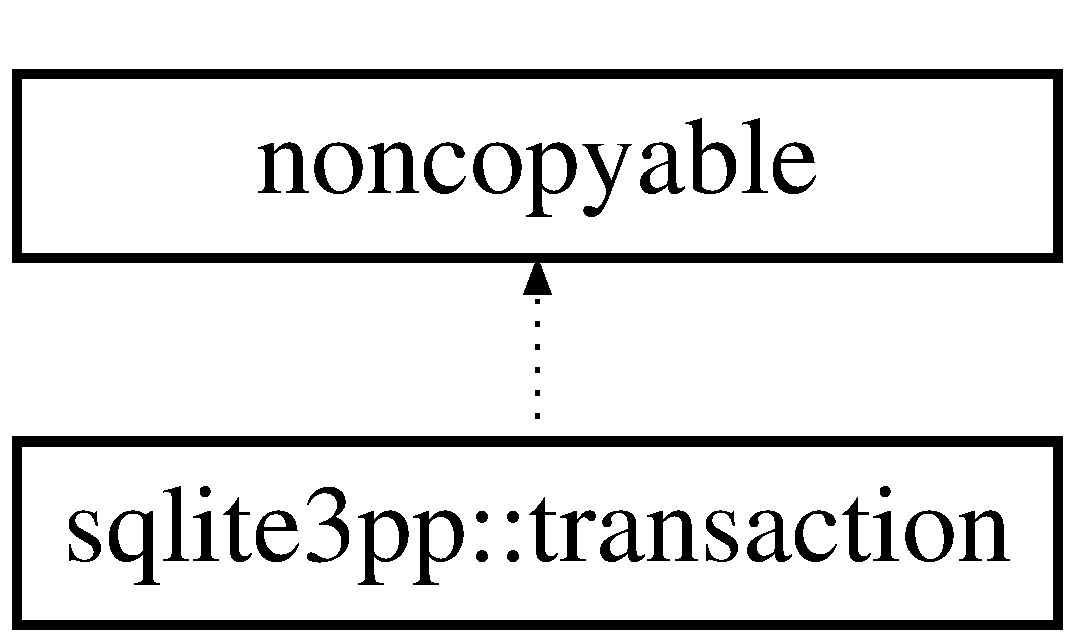
\includegraphics[height=2.000000cm]{classsqlite3pp_1_1transaction}
\end{center}
\end{figure}
\subsection*{Public Member Functions}
\begin{DoxyCompactItemize}
\item 
\hypertarget{classsqlite3pp_1_1transaction_ad5cdb7bd3463e42b1764397b11cdfd0e}{{\bfseries transaction} (\hyperlink{classsqlite3pp_1_1database}{database} \&db, bool fcommit=false, bool freserve=false)}\label{classsqlite3pp_1_1transaction_ad5cdb7bd3463e42b1764397b11cdfd0e}

\item 
\hypertarget{classsqlite3pp_1_1transaction_abe9d351fd9cdd99b5f1e418e79df687f}{int {\bfseries commit} ()}\label{classsqlite3pp_1_1transaction_abe9d351fd9cdd99b5f1e418e79df687f}

\item 
\hypertarget{classsqlite3pp_1_1transaction_a319bebdd5cb0a9dce97da274ff5d139d}{int {\bfseries rollback} ()}\label{classsqlite3pp_1_1transaction_a319bebdd5cb0a9dce97da274ff5d139d}

\end{DoxyCompactItemize}


The documentation for this class was generated from the following files\-:\begin{DoxyCompactItemize}
\item 
sqlite3pp.\-h\item 
sqlite3pp.\-cpp\end{DoxyCompactItemize}

%--- End generated contents ---

% Index
\newpage
\phantomsection
\addcontentsline{toc}{part}{Index}
\printindex

\end{document}
